\documentclass[12pt,a4paper,leqno]{report}

%\usepackage[ansinew]{inputenc}
\usepackage[utf8]{inputenc}
\usepackage[T1]{fontenc}
\usepackage[finnish]{babel}
\usepackage{amsthm}
\usepackage{amsfonts}         
\usepackage{amsmath}
\usepackage{amssymb}
\usepackage{enumerate}
\usepackage{enumitem}
\usepackage{tikz}
\usetikzlibrary{matrix}

\newcommand{\R}{\mathbb{R}}
\newcommand{\C}{\mathbb{C}}
\newcommand{\Q}{\mathbb{Q}}
\newcommand{\N}{\mathbb{N}}
\newcommand{\No}{\mathbb{N}_0}
\newcommand{\Z}{\mathbb{Z}}
\newcommand{\U}{\,\mathcal{U}}
\newcommand{\T}{\mathcal{T}}
\newcommand{\Pot}{\mathcal{P}}
\newcommand{\F}{\mathcal{F}}
\newcommand{\B}{\mathcal{B}}
\newcommand{\diam}{\operatorname{diam}}

\theoremstyle{plain}
\newtheorem{lause}[equation]{Lause}
\newtheorem{lem}[equation]{Lemma}
\newtheorem{prop}[equation]{Propositio}
\newtheorem{kor}[equation]{Korollaari}

\theoremstyle{definition}
\newtheorem{maar}[equation]{Määritelmä}
\newtheorem{konj}[equation]{Konjektuuri}
\newtheorem{esim}[equation]{Esimerkki}

\theoremstyle{remark}
\newtheorem{huom}[equation]{Huomautus}
\newtheorem{sopimus}[equation]{Sopimus}

\pagestyle{plain}
\setcounter{page}{1}
\addtolength{\hoffset}{-1.15cm}
\addtolength{\textwidth}{2.3cm}
\addtolength{\voffset}{0.45cm}
\addtolength{\textheight}{-0.9cm}

\begin{document}

%\maketitle
\begin{titlepage}
  \setlength{\parindent}{0mm}
  \sloppy
  \large \textsc{Helsingin Yliopisto \\
                 Matemaattis-luonnontieteellinen tiedekunta \\
                 Matematiikan ja tilastotieteen laitos}
  \vspace{5mm}
  \hrule height3pt
  \vspace{20mm}
  \begin{center}
    \large Pro gradu -tutkielma
    \linebreak \vfill   
    \huge \textbf{Stone–Čech kompaktisointi}
    \vspace{20mm} \linebreak
    \Large Pekka Keipi \linebreak
    %\normalsize 0000000  % opiskelijanumero
    \vfill
  \end{center}
  \hrule height2pt
  \vspace{15mm}
  Ohjaaja: Erik Elfving
  \hfill
  %18.11.2016    % päivämäärä (esim. 2.2.2002)
  \today
\end{titlepage}

\tableofcontents

\chapter{Johdanto}\label{johd}

%Nicolas Bourbaki is the pseudonym for a group of mathematicians that included Henri Cartan, Claude Chevalley, Jean Dieudonne, and Andres Weil. Mostly French, they emphasized an axiomatic and abstract treatment on all aspects of modern mathematics in Elements de mathematique. The first volume of Elements appeared in 1939. Subsequently, a wide variety of topics have been covered, including works on set theory, algebra, general topology, functions of a real variable, topological vector spaces, and integration. One of the goals of the Bourbaki series is to make the logical structure of mathematical concepts as transparent and intelligible as possible. The books listed below are typical of volumes written in the Bourbaki spirit and now available in English.

Tämän tutkielman tavoitteena on esitellä ja konstruoida Stone–Čech kompaktisointi täysin säännöllisille avaruuksille. Tutkielmassa esitellään myös uniforminen avaruus ja käsitellään tämän yhteyttä pseudometriikoihin. 

Venäläinen matemaatikko Andrey Tihonov (1906-1993) viittasi Stone–Čech kompaktisointina myöhemmin tunnettuun tulokseen jo vuonna 1930. 
Tulos pohjautuukin juuri Tihonovin työhön ja osa tutkielmassa käytetyistä aputuloksista on alun perin Tihonovin todistamia. 
Amerikkalainen Marshall Stone (1903-1989) ja tšekkiläinen Eduard Čech (1893-1960) todistivat vuonna 1937 Stone–Čech kompaktisoinnin olemassaolon ja sen ominaisuuksia. 
Čech tunnetaan saavutuksistaan algebrallisen topologian parissa, muun muassa hänen mukaansa nimetty Čech-kohomologia. 
Stone on puolestaan tunnettu muun muassa työstään funktionaali analyysin ja boolean algebran parissa. 

Tutkielman alussa käydään läpi käytettäviä topologiaan ja joukkomerkintöihin liittyviä käsitteitä ja merkintätapoja. 
Lukijan oletetaan tuntevan yleisen topologisen avaruuden määritelmä ja tähän liittyviä perustuloksia. 

%Täysin säännöllinen avaruus määritellään uniformisen avaruuden avulla. 
Peruskäsitteiden jälkeen esitellään uniforminen avaruus, eli 
%Uniforminen avaruus on 
topologinen avaruus, johon on lisätty uniforminen rakenne. 
Tämä rakenne mahdollistaa muun muassa täydellisyyden ja tasaisen jatkuvuuden määrittelyn ilman metriikkaa. 
Hausdorff uniformisoituvalle avaruudelle, eli täysin säännölliselle avaruudelle voidaan konstruoida Stone–Čech kompaktisointi.

%Stone–Čech kompaktisointi voidaan konstruoida useilla keskenään yhtäpitävillä tavoilla, muun muassa ultrafilttereillä tai $C^*$-algebroilla. 
Tässä tutkielmassa Stone–Čech kompaktisointi konstruoidaan käyttäen upotusta yksikkövälien tuloon. 
Tulos voitaisiin konstruoida yhtäpitävästi myös muilla tavoilla, muun muassa ultrafilttereillä tai $C^*$-algebroilla. 
Näitä muita tapoja emme kuitenkaan tässä työssä käsittele. 


\chapter{Esitietoja}
Tässä luvussa käydään läpi tutkielmassa käytettäviä topologiaan ja joukkomerkintöihin liittyviä käsitteitä ja merkintätapoja. 
Perusteellisemmin näistä aiheesta löytyy muun muassa kirjoista 
\cite{Eom1} ja \cite{Topo2}.
%General Topology Part 1 \cite{Eom1} ja Topologia II \cite{Topo2}.
\begin{sopimus}
Käytämme koko tutkielman ajan merkintää $\R_+=\{a\in\R\mid a>0\}$.
\end{sopimus}
\begin{maar}
Olkoon $X$ joukko ja $V$ ja $W$ karteesisen tulon $X\times X$ osajoukkoja.
Merkitään tällöin %joukkoilla $V$ ja $W$ 
seuraavasti: 
$$V\circ W=\{(x,z)\mid \text{on olemassa sellainen }y \in X,\text{ jolla }(x,y)\in V\text{ ja }(y,z)\in W\},$$ 
%$V\circ W=\{(x,z)\mid$ on olemassa sellainen $y \in X$, jolla $(x,y)\in V$ ja $(y,z)\in W\},$ 
$W^2=W\circ W$ ja $W^n=W\circ W^{n-1}$.
\end{maar}
\begin{maar}
Topologisen avaruuden $(X,\T)$ osajoukko $A\subset X$ on avoin, 
jos se on kokoelman $\T\subset\Pot(X)$ alkio.
\end{maar}
\begin{maar}%Topo2 ?
%\emph{Ympäristö.} 
%Olkoon $(X,\T)$ topologinen avaruus ja $x\in X$ alkio. 
%Osa\-jouk\-ko $A\subset X$, johon alkio $x$ kuuluu, on alkion $x$ \emph{ympäristö}, 
%jos on olemassa avoin osajoukko $B\subset X $, joka sisältää osajoukon $A$.
Topologisen avaruuden $(X,\T)$ 
osa\-jouk\-ko $A\subset X$ on alkion $x$ \emph{ympäristö}, 
jos on olemassa sellainen avoin osajoukko $B\subset X $, jolla $x\in B\subset A$.
\end{maar}
\begin{huom}
%Topologisen avaruuden $(X,\T)$ avoin osajoukko $A\subset X$ on 
%jokaisen alkionsa $x\in A$ ympäristö.
Topologisen avaruuden avoin osajoukko on 
jokaisen alkionsa ympäristö.
\end{huom}
\begin{maar}%Topo2 2.14
\emph{Ympäristökanta.} 
Olkoon $(X,\T)$ topologinen avaruus ja $x\in X$ alkio. 
Kokoelma $B(x)$ alkion $x$ ympäristöjä on alkion $x$ \emph{ympäristökanta} 
(topologiassa $\T$), jos jokainen alkion $x$ ympäristö sisältää 
kokoelman $B(x)$ jonkin jäsenen. 
\end{maar}
%\begin{maar}
%Olkoon $(X,\T)$ topologinen avaruus, $x\in X$ alkio ja . 
%Alkion $x$ kaikkien ympäristöjen kokoelmalle pätee seuraavat ehdot: 
%\begin{enumerate} [label=(V\arabic*),ref=(V\arabic*)]
%\item Jos 
%\end{enumerate} 
%\end{maar}
\begin{huom}\label{kaikki_ystöt}
Topologisen avaruuden $(X,\T)$ alkion $x\in X$ kaikkien ympäristöjen kokoelma $B(x)$ on alkion $x$ ympäristökanta.
\end{huom}
\begin{esim}
Jos joukkoperhe $B\subset\Pot(X)$ on avaruuden $(X,\T)$ kanta ja 
$x\in X$ alkio, niin joukko 
$B(x)=\{A\mid x\in A\in B\}$ on alkion $x$ eräs ympäristökanta.
Käänteisesti, jos jokaisella alkiolla $x\in X$ on annettu ympäristökanta 
$B(x)$ avaruudessa $(X,\T)$, niin kokoelma $\bigcup\{B(x)\mid x\in X\}$ 
on avaruuden $(X,\T)$ kanta.
\end{esim}
%\begin{maar}
%Joukon $X$ peite $A$ virittää yksikäsitteisesti
%\end{maar}
\begin{lause}
Olkoon $A$ joukon $X$ peite. Tällöin $A$ on joukon $X$ erään topologian $\T$ esikanta. 
Lisäksi $\T$ on karkein niistä joukon $X$ topologioista, joilla $A\subset\T$. 
Tämä topologia $\T$ on peitteen $A$ yksikäsitteisesti määräämä, ja sitä sanotaan peitteen $A$ virittämäksi joukon $X$ topologiaksi.
\begin{proof}
Topologia II \cite{Topo2} Lause 2.19.
%topo2 2.19
\end{proof}
\end{lause}
\begin{maar}
\emph{Topologioiden vertailu.}
Olkoon $X$ joukko ja $\T_1$ ja $\T_2$ topologioita joukolle $X$.
Topologia $\T_2$ on karkeampi kuin topologia $\T_1$, 
jos jokaisella $ U\in\T_2$ pätee $ U\in\T_1$, eli $ \T_2\subset\T_1$. 
Tällöin $\T_1$ on hienompi kuin $\T_2$.
\end{maar}
\chapter{Uniformiset rakenteet}
%Tässä luvussa tutustutaan uniformisiin rakenteisiin. 
Topologian kannalta kahden eri pisteen etäisyyttä toisiinsa voidaan tutkia lähinnä siltä kannalta, että kuuluvatko ne toistensa jokaiseen ympäristöön, eli ovatko ne hyvin lähellä toisiaan. 
Metriikka puolestaan antaa jokaiselle kahdelle pisteelle tarkan etäisyyden. 
Topologian ja metriikan väliltä löytyy uniforminen rakenne \cite[luku~II]{Eom1}, 
jossa vertaillaan pisteparien etäisyyksiä toisiinsa. 
Tässä luvussa tutustutaan uniformisiin rakenteisiin. 
Lisäksi käsitellään uniformisen rakenteen yhteyttä topologiaan. 
%\\
%\\
%Merkitään joukkoilla $V$ ja $W$ seuraavasti: $$V\circ W=\{(x,z)\mid \text{ on olemassa sellainen }y \in X\text{ jolla }(x,y)\in V\text{ ja }(y,z)\in W\}$$ ja $W^2=W\circ W$.
\begin{maar}\label{uniformi_maar}
\emph{Uniforminen rakenne} (tai \emph{uniformiteetti}) joukolle $X$ annetaan karteesisen tulon $X\times X$ potenssijoukon $\Pot(X\times X)$ osajoukkona $\U$, jolle pätee %kaikilla $V\in \U$
\begin{enumerate} [label=(U\arabic*),ref=(U\arabic*)]
\item\label{F_I} Jos $V\in \U$ ja $V\subset W\subset X\times X$ niin $ W\in\U$,
\item\label{F_II} Jokainen äärellinen leikkaus joukon $\U$ alkioista kuuluu joukkoon $\U$,
\item\label{U_I} Joukko $\{(x,x)\mid x\in X\}$ on jokaisen joukon $V\in\U$ osajoukko,
\item\label{U_II} Jos $V\in\U$, niin $V^{-1}=\{(y,x)\mid (x,y)\in V\}\in\U$,
\item\label{U_III} Jos $V\in \U$, niin on olemassa sellainen $W\in \U$, jolla $ W^2\subset V$.%$ W\circ W\subset V$.
\end{enumerate}
Uniformisen rakenteen muodostavia joukkoja $ V\in\U$ sanotaan uniformiteetin $\U$ lähistöiksi. 
Uniformiteetilla $\U$ varustettua joukkoa $X$ sanotaan uniformiseksi avaruudeksi.
Uniformista avaruutta voidaan myös merkitä parina $(X,\U)$.
\end{maar}
\begin{huom}\label{V-close}
Uniformiteetin $\U$ lähistöön (entourage) $V\in\U $ kuuluvan 
pisteparin $(x,y)\in V$ pisteiden $x,y\in X$ sanotaan olevan $V-$lähellä, 
tarpeeksi lähellä tai mielivaltaisen lähellä toisiaan.
\end{huom}
\begin{huom}\label{UaHuom}
%Mikäli muut ehdot pätevät, voidaan ehdot (U$\ref{U_II}$) ja (U$\ref{U_III}$) korvata yhtäpitävällä ehdolla 
Mikäli muut ehdot pätevät, voidaan ehdot \ref{U_II} ja \ref{U_III} korvata yhtäpitävällä ehdolla: 
\begin{enumerate} [label=(Ua),ref=(Ua)]
%\item[(U$\ref{U_II}$a)] \label{Uaehto} 
\item \label{Uaehto} 
%\item[(Ua)] \label{Uaehto} 
Jos $V\in \U$, niin on olemassa sellainen $W\in \U$, jolla $ W\circ W^{-1}\subset V$.
\end{enumerate}
%Ehto (U$\ref{U_II}$\ref{Uaehto}) seuraa
%ehdoista (U$\ref{U_II}$) ja (U$\ref{U_III}$), sillä\dots
%
%Ehdot 
\end{huom}
\begin{huom}
%Jos joukko $X$ on tyhjä, niin ehdon (U$\ref{U_I}$) 
%Jos joukko $X$ on tyhjä, niin ehdon \ref{U_I} 
%nojalla joukon $X$ uniformiteetti $\U$ on tyhjä. Erityisesti kokoelma $\{\emptyset\}$ on joukon $X$ ainoa ehdot täyttävä uniformiteetti, jos joukko $X$ on tyhjä.
Kokoelma $\{\emptyset\}$ on ainoa uniformiteetin ehdot täyttävä kokoelma tyhjälle joukolle.
\end{huom}
\begin{maar}\label{uniformi_kanta}
Olkoon $X$ joukko ja kokoelma $\U\subset \Pot (X\times X)$ uniformiteetti 
joukolle $X$. Tällöin lähistöjen joukko $B\subset \U$ on 
uniformiteetin $\U$ \emph{kanta}, jos jokaiselle lähistölle $V\in\U$ löytyy 
kannan alkio $W\in B$, jolla pätee $W\subset V$.
\end{maar}
%\begin{kor}
%Uniformiteetin kannas
%\end{kor}
\begin{lause}\label{uniformin kannan maar}
Kantalause. 
Olkoon $X$ joukko. 
%Olkoon joukko $X$ varustettu uniformiteetilla $\U$. 
%Kokoelma $B\subset \U$ on uniformiteetin $\U$ kanta, 
Kokoelma $B\subset \Pot (X\times X)$ on joukon $X$ erään uniformiteetin kanta, 
jos kokoelmalle $B$ pätee
%Olkoon $X$ joukko ja $B\subset \Pot (X\times X)$ sellainen joukko, jolla pätee
\begin{enumerate} [label=(B\arabic*)]
\item\label{B_I} Jos $V_1,V_2\in B$ niin on olemassa sellainen $V_3\in B$, jolla $V_3\subset V_1\cap V_2$,
\item\label{U'_I} Joukko $\{(x,x)\mid x\in X\}$ on jokaisen joukon $V\in B$ osajoukko,
\item\label{U'_II} Jos $V\in B$, niin on olemassa sellainen $V'\in B$, jolla $V'\subset V^{-1}%=\{(y,x)\mid (x,y)\in V\}
$,
\item\label{U'_III} Jos $V\in B$, niin on olemassa sellainen $W\in B$, jolla $ W^2\subset V$.%$ W\circ W\subset V$.
\end{enumerate}
\begin{proof}
%Olkoon joukko $X$ varustettu uniformiteetilla $\U$. 
Olkoon $X$ joukko ja $B\subset \Pot (X\times X)$ sellainen kokoelma, 
jolle pätevät ehdot \ref{B_I}-\ref{U'_III}. %karteesisen tulon $X\times X$ osajoukkoja. 
Tällöin olkoon 
$$\U_B=\{W\subset X\times X\mid V\subset W\text{ jollain } V\in B\}$$ 
joukko. 
%$\U_B\subset\Pot (X\times X)$ sellainen kokoelma, 
%jonka alkioina ovat kaikki sellaiset joukot $V'\subset$
%jolla pätee seuraava ehto: Jos $V\in B$ ja $V\subset W\subset X\times X$ niin $ W\in\U_B$. 
Joukon $\U_B$ määrittelystä seuraa, 
että jokaiselle alkiolle $W\in\U_B$ löytyy 
kannan alkio $V\in B$, jolla pätee $V\subset W$. 
Lisäksi $ B\subset\U_B$.
Näin ollen riittää tarkistaa, että $\U_B$ on uniformiteetti. 
%Tällöin olkoon 
%%$$B'=\{V\subset X\times X\mid \text{on olemassa } U\in B\}$$ 
%$\U\subset\Pot (X\times X)$ karkein sellainen uniformiteetti, jolla $B\subset \U$.
%%jolla pätee seuraava ehto: Jos $V\in B$ ja $V\subset W\subset X\times X$ niin $ W\in\U_B$. 
%%Ehdosta seuraa $ B\subset\U_B$ ja että jokaiselle lähistölle $W\in\U$ löytyy 
%%kannan alkio $V\in B$, jolla pätee $V\subset W$. 
%%Näin ollen riittää tarkistaa, että $\U_B$ on uniformiteetti. 
Käydään läpi uniformiteetin määritelmän \ref{uniformi_maar} ehdot:
\begin{enumerate} 
\item[\ref{F_I}] 
Jos $W\in \U_B$, niin on olemassa sellainen $V\in B$, jolla pätee $V\subset W$. 
Toisaalta jos osajoukolle $W'\subset X\times X$ pätee $V\subset W \subset W'$, 
niin $W'\in\U_B$. \\
Siis jos $W\in \U_B$ ja $W\subset W'\subset X\times X$ niin $ W'\in\U_B$.
%Jos $V\in \U_B$ ja $V\subset W\subset X\times X$ 
%niin joukon $\U_B$ määrittelyn nojalla $ W\in\U_B$,
%Jos $V\in \U$ ja $V\subset W\subset X\times X$ niin $ W\in\U$,
\item[\ref{F_II}] Olkoon $W\in\U_B$ ja $W'\in\U_B$ joukkoja. 
Joukon $\U_B$ määrittelyn nojalla tällöin on olemassa 
sellaiset $V\in B$ ja $V'\in B$, 
joille pätee $V\subset W$ ja $V'\subset W'$ ja 
erityisesti $V\cap V'\subset W\cap W'$. 
Edelleen ehdon \ref{B_I} nojalla on olemassa sellainen $V''\in B$, 
jolle pätee $V''\subset V\cap V'$ ja siis $V''\subset W\cap W'$. 
Näin ollen leikkaus $W\cap W'$ kuuluu kokoelmaan $\U_B$. 
Lisäksi joukoiksi $W$ ja $W'$ voidaan valita mielivaltaisia kokoelman $\U_B$ alkioita, 
joten induktiivisesti jokainen äärellinen leikkaus joukon $\U_B$ alkioista kuuluu joukkoon $\U_B$.
\item[\ref{U_I}] 
%Joukon $\U_B$ määrittelystä seuraa, 
%että j
Jokaiselle alkiolle $W\in\U_B$ löytyy 
kannan alkio $V\in B$, jolla pätee $V\subset W$. 
%Näin ollen ehdon \ref{U'_I} nojalla $\{(x,x)\mid x\in X\}\subset V\subset W$. 
Ehdon \ref{U'_I} nojalla $\{(x,x)\mid x\in X\}\subset V$, 
joten $\{(x,x)\mid x\in X\}\subset W$.
\item[\ref{U_II}] Olkoon $W\in\U_B$. 
Tällöin joukon $\U_B$ määrittelyn nojalla on olemassa sellainen $V\in B$, 
jolla $V\subset W$. %(Jos $W\in B$, niin voidaan valita $V=W$.) 
%Tällöin pätee joko $V\in B$ tai $V\not\in B$. 
%Jos $V\in B$, niin ehdon \ref{U'_II} nojalla on olemassa sellainen $V'\in B$, 
%jolla $V'\subset V^{-1}$. 
%Näin ollen joukon $\U_B$ määrittelyn nojalla $V^{-1}\in\U_B$. 
%Jos $V\not\in B$, niin 
Tällöin ehdon \ref{U'_II} nojalla joukolle $V$ on olemassa sellainen $V'\in B$, 
jolla $V'\subset V^{-1}$. 
Näin ollen joukon $\U_B$ määrittelyn nojalla $V^{-1}\in\U_B$ ja 
edelleen $W^{-1}\in\U_B$. 
%Nyt $V\subset W$ ja $V^{-1}\in\U_B $
\item[\ref{U_III}] Olkoon $W\in\U_B$. 
Tällöin joukon $\U_B$ määrittelyn nojalla on olemassa sellainen $V'\in B$, 
jolla $V'\subset W$. 
Ehdon \ref{U'_III} nojalla on olemassa sellainen $V\in B$, jolla $ V^2\subset V'$. 
Joukon $\U_B$ määrittelyn nojalla tällöin $V\in \U_B$ ja siis $ V^2\subset W$.
%Jos $V\in \U$, niin on olemassa sellainen $W\in \U$, jolla $ W^2\subset V$.
\end{enumerate}
\end{proof}
\end{lause}
\begin{lause}
%\emph{Uniformisen avaruuden topologia.}
Uniformisen avaruuden topologia.
Olkoon joukko $X$ varustettu uniformiteetilla $\U$.
Olkoon $x\in X$ 
alkio ja $V\in\U$ lähistö. 
%alkio, $V\in\U$ lähistö ja $B\subset\U$ uniformiteetin $\U$ kanta. 
Olkoon tällöin %$V(x)\subset X$,
\begin{equation*}V(x)=\{ y\in X\mid (x,y)\in V \}
\quad\text{ ja }\quad
B(x)=\{ V(x)\mid V\in\U \}
\end{equation*}
joukkoja.
Uniformiteetti $\U$ määrää topologian joukolle $X$ niin, 
että joukko $V(x)$ on (lähistön $V$ määräämä) ympäristö 
alkiolle $x$ ja joukko $B(x)$ on alkion $x$ 
ympäristökanta kyseisessä topologiassa.
\begin{proof}
Olkoon joukko $X$ varustettu uniformiteetilla $\U$, 
$x\in X$ alkio ja $V\in\U$ lähistö avaruudessa $X$. Lisäksi olkoot joukot $V(x)$ ja $B(x)$ kuten edellä. 
%
Joukko $V(x)$ on epätyhjä, sillä $x\in V(x)$.
%Alkio $x$ kuuluu joukkoon $V(x)$, joten joukko $V(x)$ on epätyhjä. 
%Jokaiselle lähistölle $V,W\in\U$ pätee 
%\begin{align*}
%V(x)\cup W(x) =&\{ y\in X\mid (x,y)\in V \text{ tai } (x,y)\in W \}\\
%=&\{ y\in X\mid (x,y)\in V\cup W \}
%\in B(x),
%\end{align*} 
%ja 
Olkoon $W\in\U$ lähistö, jolloin $W(x)$ on alkion $x$ ympäristö. 
Alkion $x$ ympäristöille $V(x)$ ja $W(x)$ pätee
\begin{align*}
V(x)\cap W(x) =&\{ y\in X\mid (x,y)\in V \text{ ja } (x,y)\in W \}\\
=&\{ y\in X\mid (x,y)\in V\cap W \}
\in B(x),
\end{align*} 
%sillä määritelmän \ref{uniformi_maar} ehtojen \ref{F_I} ja \ref{F_II} nojalla $ V\cup W \in B$ ja $ V\cap W \in B$. 
sillä määritelmän \ref{uniformi_maar} ehdon \ref{F_II} 
nojalla pätee $ V\cap W \in \U$. 
%Olkoon lisäksi $U\subset X$ joukko, jolle pätee $V(x)\subset U$. 
%Nyt joukkoa $U$ vastaa jokin $U'\in X\times X$, 
%jolla pätee  $U'\in \U$.
Ehdosta \ref{F_I} seuraa, että 
joukko $B(x)$ on alkion $x$ kaikkien ympäristöjen joukko ja siten 
huomautuksen \ref{kaikki_ystöt} nojalla ympäristökanta.
%Tällöin on olemassa yksikäsitteinen topologia, jossa $B(x)$ on alkion $x$ kaikkien ympäristöjen joukko.\cite{Eom1}
%yhdisteen kohdassa tarvitaan yleisempi tapaus. ehto V_4 puuttuu sivu19 Eom1
\end{proof}
\end{lause}
\begin{huom}\label{unif_indusoitu_topo}
Uniformiteetin määräämää topologiaa sanotaan uniformiteetin indusoimaksi topologiaksi.
\end{huom}
\begin{maar}\label{tasaisesti_jatkuva}
%Uniformisesti jatkuvat kuvaukset. 
Olkoot $X$ ja $X'$ uniformeja avaruuksia 
ja $f\colon X\rightarrow X'$ kuvaus.
Kuvaus $f$ on \emph{tasaisesti jatkuva} (uniformly continuous), jos jokaiselle avaruuden $X'$ lähistölle $V'$ on olemassa avaruuden $X$ lähistö $V$ niin, että jokaiselle $(x,y)\in V$ pätee $(f(x),f(y))\in V'$. 
%Toisin sanoen jokaiselle avaruuden $X'$ lähistölle $V'$ on olemassa.
\end{maar}
\begin{kor}\label{uniformi alkukuva}
Olkoot $X$ ja $X'$ uniformeja avaruuksia 
ja $f\colon X\rightarrow X'$ tasaisesti jatkuva kuvaus. 
Olkoon $g\colon X\times X\rightarrow X'\times X'$ %sellainen 
kuvaus, jolla pätee $g(x,y)=(f(x),f(y))$ kaikilla $x,y\in X$. 
Tällöin jos $V'$ on avaruuden $X'$ lähistö, niin alkukuva $g^{\leftarrow}V'$ on avaruuden $X$ lähistö.
\begin{proof}
Korollaari on suora seuraus määritelmästä \ref{tasaisesti_jatkuva} ja uniformiteetin määritelmän \ref{uniformi_maar} ehdosta \ref{F_I}.
\end{proof}
\end{kor}
\begin{lause}
%Jokainen tasaisesti jatkuva kuvaus on jatkuva myös lähtö- ja maalijoukkojen uniformien määräämien topologioiden suhteen.
Olkoot $X$ ja $X'$ uniformeja avaruuksia 
ja $f\colon X\rightarrow X'$ tasaisesti jatkuva kuvaus. 
Tällöin kuvaus $f$ on jatkuva, %myös topologioiden kannalta, 
kun varustetaan joukot $X$ ja $Y$ uniformiteettiensa indusoimilla topologioilla.
\begin{proof}
Olkoot $X$ ja $X'$ uniformeja avaruuksia 
ja $f\colon X\rightarrow X'$ tasaisesti jatkuva kuvaus. 
Olkoon $g\colon X\times X\rightarrow X'\times X'$ %sellainen 
kuvaus, jolla pätee $g(x,y)=(f(x),f(y))$ kaikilla $x,y\in X$. 
Olkoon $V'$ avaruuden $X'$ lähistö ja $x'\in X'$ alkio. 
Avaruuden $X'$ uniformiteetin indusoimassa topologiassa kaava 
$$V'(x')=\{ y'\in X'\mid (x',y')\in V'\}$$
määrää alkion $x'$ ympäristön avaruudessa $X$.
Korollaarin \ref{uniformi alkukuva} mukaan lähistön $V'$ alkukuva $g^{\leftarrow}V'$ on avaruuden $X$ lähistö.
Olkoon nyt $x\in X$ sellainen alkio, jolla $f(x)=x'$.
Tällöin joukko $(g^{\leftarrow}V')(x)$ on alkion $x$ ympäristö. 
%Olkoon nyt $x\in g^\leftarrow (x')$ alkio, jolloin 
Erityisesti ympäristö $(g^{\leftarrow}V')(x)$ kuvautuu ympäristöön $V'(x')$, 
sillä ehdosta $(x,y)\in g^\leftarrow V'$ seuraa $(x',f(y))\in V' $ kaikilla $y\in X$.
%
%Tällöin olkoon $x\in X$ sellainen alkio, jolla $f(x)=x'$. 
%Nyt koska $g^{\leftarrow}V'$ on avaruuden $X$ lähistö, 
%niin $g^{\leftarrow}V'(x)$ on alkion $x'$ alkukuvaan $g^{\leftarrow}(x')$ kuuluvan alkion $x$ ympäristö. 
%
%Tällöin koska $g^{\leftarrow}V'$ on avaruuden $X$ lähistö, niin $g^{\leftarrow}V'(g^{\leftarrow}(x'))$ on alkion $x'$ alkukuvan $g^{\leftarrow}(x')\in X$ ympäristö. 
%erikseen 1-käs? eli alkukuva ympäristöstä lähistön sijaan?

Siis ympäristön alkukuva on ympäristö ja siten tasaisesti jatkuva kuvaus on jatkuva.
\end{proof}
\end{lause}
\begin{lause}
Olkoot $X$, $X'$ ja $X''$ uniformeja avaruuksia 
ja $f\colon X\rightarrow X'$ ja $g\colon X'\rightarrow X''$ 
tasaisesti jatkuvia kuvauksia. 
Tällöin yhdistetty kuvaus $g\circ f\colon X\rightarrow X''$ on tasaisesti jatkuva.
\begin{proof}
Olkoot $X$, $X'$ ja $X''$ uniformeja avaruuksia, 
$f\colon X\rightarrow X'$ ja $g\colon X'\rightarrow X''$ tasaisesti jatkuvia kuvauksia ja 
$V''$ avaruuden $X''$ lähistö. 
Tällöin tasaisesti jatkuvan kuvauksen määritelmän nojalla 
on olemassa avaruuden $X'$ lähistö $V'$, 
jolla jokaisella $(x',y')\in V'$ pätee $ (g(x'),g(y'))\in V''$.
Edelleen lähistölle $V'$ on olemassa avaruuden $X$ lähistö $V$, 
jolla jokaisella $(x,y)\in V$ pätee $ (f(x),f(y))\in V'$.
Näin ollen lähistölle $V''$ on olemassa lähistö $V$, 
jolla jokaisella $(x,y)\in V$ pätee $ (g(f(x)),g(f(y)))\in V''$, 
%ja koska yhdistetyllä kuvauksella pätee $g(f(x))=(g\circ f)(x)$, 
%niin jokaisella $(x,y)\in V$ pätee 
eli $ ((g\circ f)(x),(g\circ f)(y))\in V''$.
%Yhdistetyllä kuvauksella $g\circ f\colon X\rightarrow X''$ 
%pätee $(g\circ f)(x)$ 

Siis yhdistetty kuvaus $g\circ f\colon X\rightarrow X''$ on tasaisesti jatkuva.
\end{proof}
\end{lause}
\begin{maar}
Olkoot $X$ ja $X'$ uniformeja avaruuksia 
ja $f\colon X\rightarrow X'$ bijektiivinen kuvaus. 
Kuvaus $f$ on \emph{isomorfismi}, jos sekä kuvaus $f$ että sen 
käänteiskuvaus $f^{-1}$ ovat tasaisesti jatkuvia.
\end{maar}
\begin{maar}\label{uniformi_vertailu}
\emph{Uniformiteettien vertailu.} 
Olkoon $X$ joukko ja $\U_1$ ja $\U_2$ uniformiteetteja joukolle $X$. 
Uniformiteetti $\U_2$ on karkeampi kuin uniformiteetti $\U_1$, 
jos identtinen kuvaus $id\colon (X,\U_1)\rightarrow (X,\U_2)$ on tasaisesti jatkuva. Tällöin $\U_1$ on hienompi kuin $\U_2$. 

Jos lisäksi pätee $\U_1\neq\U_2$, niin $\U_1$ on aidosti hienompi kuin $\U_2$ ja vastaavasti $\U_2$ on aidosti karkeampi kuin $\U_1$. 
Sanotaan, että kahta uniformiteettia $\U_1$ ja $\U_2$ voidaan vertailla, 
jos $\U_1$ on hienompi tai karkeampi kuin $\U_2$. 
Uniformiteeteille $\U_1$ ja $\U_2$ pätee $\U_1=\U_2$, 
jos $\U_1$ on sekä hienompi että karkeampi kuin $\U_2$.
\end{maar}
\begin{kor}
Olkoon $X$ joukko ja $\U_1$ ja $\U_2$ uniformiteetteja joukolle $X$. 
Uniformiteetti $\U_1$ on hienompi kuin uniformiteetti $\U_2$ jos ja vain jos jokaisella lähistöllä $V\in\U_2$ pätee $V\in\U_1$.
\end{kor}
\begin{kor}
Olkoon $X$ joukko, $\U_1$ ja $\U_2$ uniformiteetteja joukolle $X$ ja 
$\U_1$ on hienompi kuin $\U_2$. 
Tällöin uniformiteetin $\U_1$ indusoima topologia on hienompi kuin 
uniformiteetin $\U_2$ indusoima topologia.
\end{kor}
%\begin{maar}\label{kuvausperheen indusoima maar}
%Olkoon $X$ joukko ja $(Y_i,\U_i)$ uniforminen avaruus jokaisella $i\in I$, jollain indeksijoukolla $I$. 
%Olkoon $f_i\colon X\rightarrow Y_i$ kuvaus jokaisella $i\in I$ ja  
%$g_i\colon X\times X\rightarrow Y_i\times Y_i$ kuvaus, jolla $g_i(x,y)=(f_i(x), f_i(y))$ kaikilla $x,y\in X$ ja 
%$i\in I$.
%Tällöin joukko 
%$$B=\left\{\bigcap_{i\in J}g^{\leftarrow}_{i}(V_{i})
%\mid J\subset I\text{ äärellinen},V_{i} \in\U_{i}\text{ kaikilla } i\in J\right\}$$
%on kuvausperheen $(f_i)_{i\in I}$ indusoiman uniformiteetin kanta.
%%on kanta eräälle avaruuden $X$ uniformiteetille $\U$. 
%%Kyseistä uniformiteettia $\U$ sanotaan 
%%%kuvausten $f_i$, tai 
%%kuvausperheen $(f_i)_{i\in I}$ indusoimaksi uniformiteetiksi.  
%\end{maar}
\begin{lause}\label{kuvausperheen indusoima lause}
%Edellisessä määritelmässä \ref{kuvausperheen indusoima maar} annettu kuvausperheen indusoiman uniformiteetin kanta todella on uniformiteetin kanta.
%
%Olkoot $X$ ja $I$ epätyhjiä joukkoja ja $(Y_i,\U_i)$ uniforminen avaruus jokaisella $i\in I$. %, jollain indeksijoukolla $I$. 
Olkoon $X$ joukko ja $(Y_i,\U_i)$ uniforminen avaruus jokaisella $i\in I$, jollain indeksijoukolla $I$. 
%Olkoon $\U_i$ joukon $Y_i$ uniformiteetti kaikilla $i\in I$.
Olkoon $f_i\colon X\rightarrow Y_i$ kuvaus jokaisella $i\in I$ ja  
%Olkoon nyt $g_i=f_i\times f_i$ kuvaus joukolta $X\times X$ joukolle $Y_i\times Y_i$ 
%Olkoon nyt 
$g_i\colon X\times X\rightarrow Y_i\times Y_i$ kuvaus, jolla $g_i(x,y)=(f_i(x), f_i(y))$ kaikilla $x,y\in X$, 
%Olkoon $g_i=f_i\times f_i\colon X\times X\rightarrow Y_i\times Y_i$ %sellainen 
%kuvaus, jolla pätee $g(x,y)=(f_i(x),f_i(y))$ kaikilla $x,y\in X$. 
%kuvauksia 
%kaikilla 
$i\in I$.
%Olkoon 
%$(i_k)$ jono joukon $I$ alkioita ja olkoon 
%$$B=\left\{\bigcap_{k=0}^{n}g^{\leftarrow}_{i_k}(V_{i_k})
%\mid V_{i_k} \in\U_{i_k},i_k \in I,n\in\N \right\}$$
Tällöin joukko 
$$B=\left\{\bigcap_{i\in J}g^{\leftarrow}_{i}(V_{i})
\mid J\subset I\text{ äärellinen},V_{i} \in\U_{i}\text{ kaikilla } i\in J\right\}$$
%$$B=\left\{\bigcap_{j\in A}g^{\leftarrow}_{j}(V_{j})
%\mid A\subset I\text{ äärellinen},V_{j} \in\U_{j}\right\}$$
%joukko missä $\U_{j}$ on avaruuden $Y_{j}$ uniformiteetti.
%Tällöin $B$ 
on kanta eräälle avaruuden $X$ uniformiteetille $\U$. 
%Tällöin $B$ on kanta kuvausperheen $ (f_i)_{i\in I}$ 
%avaruudelle $X$ indusoimalle uniformiteetille $\U$. 
%Kyseinen uniformiteetti $\U$ on karkein niistä uniformiteeteista, 
%%ja se on karkein niistä uniformiteeteista, 
%joiden suhteen kaikki kuvaukset $f_i$ ovat tasaisesti jatkuvia.
%
%Kyseistä uniformiteettia $\U$ sanotaan 
%%kuvausten $f_i$, tai 
%kuvausperheen $(f_i)_{i\in I}$ indusoimaksi uniformiteetiksi.  
\begin{proof}
Olkoon $X$ joukko ja $(Y_i,\U_i)$ uniforminen avaruus jokaisella $i\in I$. 
%, jollain indeksijoukolla $I$. 
Olkoon lisäksi kuvaukset $f_i$ ja $g_i$ ja joukko $B$ kuten yllä.
%Olkoon $f_i\colon X\rightarrow Y_i$ kuvaus jokaisella $i\in I$ ja  
%$g_i\colon X\times X\rightarrow Y_i\times Y_i$ kuvaus, jolla $g_i(x,y)=(f_i(x), f_i(y))$ kaikilla $x,y\in X$, 
%$i\in I$.
%Joukko 
%$$B=\left\{\bigcap_{i\in A}g^{\leftarrow}_{i}(V_{i})
%\mid A\subset I\text{ äärellinen},V_{i} \in\U_{i}\text{ kaikilla } i\in I\right\}$$
%$B$ on kanta eräälle avaruuden $X$ uniformiteetille $\U$. 
Selvitetään, onko joukko $B$ uniformiteetin kanta käymällä läpi 
kantalauseen \ref{uniformin kannan maar} ehdot:
\begin{enumerate} %[label=(B\arabic*)]
\item[\ref{B_I}] 
Olkoot $U_1,U_2\in B$. 
Tällöin on olemassa äärelliset osajoukot $J_1,J_2\subset I$ 
ja lähistöt $V_i\in\U_i$ kaikilla $i\in J_1$ 
ja $V_j\in\U_j$ kaikilla $j\in J_2$, 
%ja $V_i\in\U_i$
%ja kaikilla $i\in J_2$, 
joilla 
\begin{equation*}
U_1=\bigcap_{i\in J_1}g^{\leftarrow}_{i}(V_{i})\quad\text{ ja 
 }\quad U_2=\bigcap_{j\in J_2}g^{\leftarrow}_{j}(V_{j}).
\end{equation*}
%kun $V_i\in \U_i$ kaikilla $i\in A_1$.
Yhdiste $J_1\cup J_2$ on äärellinen indeksijoukon $I$ osajoukko, 
joten 
 $$U_3=\bigcap_{j\in J_1\cup J_2}g^{\leftarrow}_{j}(V_{j})\in B$$
 ja erityisesti $U_3\subset U_1\cap U_2$.
% niin on olemassa sellainen $U_3\in B$, jolla $U_3\subset U_1\cap U_2$,
\item[\ref{U'_I}] 
Olkoon $U\in B$. Tällöin on olemassa äärellinen $J\subset I$, 
ja lähistöt $V_i\in\U_i$, kaikilla $i\in J$, 
joilla
\begin{equation*}
U=\bigcap_{i\in J}g^{\leftarrow}_{i}(V_{i}).
%,\quad\text{ jossa }V_i\in\U_i.
%,\quad V_i\in\U_i.
\end{equation*}
Jokaisella $V_i\in \U_i$ pätee $\{(y_i,y_i)\mid y_i\in Y_i\}\subset V_i$ 
ja näin ollen myös jokaisella $g_i^{\leftarrow}(V_i)$ pätee 
$\{(x,x)\mid x\in X\}\subset g_i^{\leftarrow}(V_i)$. 
%Nyt myös joukolla $U\in B$ pätee $\{(x,x)\mid x\in X\}\subset U$, 
Siis pätee $\{(x,x)\mid x\in X\}\subset U$, 
koska $U$ on leikkaus joukoista $g_i^{\leftarrow}(V_i)$.
%Joukko $\{(x,x)\mid x\in X\}$ on jokaisen joukon $V\in B$ osajoukko,
\item[\ref{U'_II}] 
Olkoon $U\in B$. Tällöin on olemassa äärellinen $J\subset I$, 
ja lähistöt $V_i\in\U_i$, kaikilla $i\in J$, 
joilla
\begin{equation*}
U=\bigcap_{i\in J}g^{\leftarrow}_{i}(V_{i}).
%,\quad\text{ jossa }V_i\in\U_i.
%,\quad V_i\in\U_i.
\end{equation*}
%Kuitenkin tällöin jokaiselle $V_i\in\U_i$ löytyy $V'_i\in\U_i$, 
%jolla 
%Kuitenkin tällöin 
Uniformiteetin määritelmän ehdon \ref{U_II} nojalla jos $V_i\in\U_i$ niin $V^{-1}_i\in\U_i$. 
%ja siis  
Näin ollen 
%Siis 
\begin{equation*}
U^{-1}=\bigcap_{i\in J}(g^{\leftarrow}_{i}(V_{i}))^{-1}
=\bigcap_{i\in J}g^{\leftarrow}_{i}(V^{-1}_{i})\in B,
%,\quad\text{ jossa }V_i\in\U_i.
%,\quad V_i\in\U_i.
\end{equation*}
%%Edelleen $V_i,V_i^{-1}\in\U_i$, joten myös $V_i\cap V_i^{-1}\in\U_i$ ja näin ollen 
%%\begin{equation*}
%%B\ni\bigcap_{i\in J}(g^{\leftarrow}_{i}(V_{i}\cap V_{i}^{-1}))
%%=\bigcap_{i\in J}g^{\leftarrow}_{i}(V_{i}\cap V_{i}^{-1})\in B.
%%%,\quad\text{ jossa }V_i\in\U_i.
%%%,\quad V_i\in\U_i.
%%\end{equation*}
%%Nyt $U\in B$ ja $U^{-1}\in B$, joten ehdon \ref{F_II} nojalla $U\cap U^{-1}\in B$. 
%Siis joukolle $ U\in B$ on löydetty 
%joukko $U^{-1}\in B$, 
jolloin vaadittu ehto pätee muodossa $U^{-1}\subset U^{-1}$.
%
%Jos $V\in B$, niin on olemassa sellainen $V'\in B$, jolla $V'\subset V^{-1}%=\{(y,x)\mid (x,y)\in V\}
%$,
\item[\ref{U'_III}] 
Olkoon $U\in B$. Tällöin on olemassa äärellinen $J\subset I$, 
ja lähistöt $V_i\in\U_i$, kaikilla $i\in J$, 
joilla
\begin{equation*}
U=\bigcap_{i\in J}g^{\leftarrow}_{i}(V_{i}).
\end{equation*}
Uniformiteetin määritelmän ehdon \ref{U_III} nojalla jos $V_i\in\U_i$ niin on olemassa sellainen $W_i\in\U_i$, jolla $W^2_i\subset V_i$. 
Olkoon 
\begin{equation*}
A=\bigcap_{i\in J}g^{\leftarrow}_{i}(W_{i}),
\end{equation*}
jolloin $A\in B$ ja näin ollen riittää osoittaa, että $A^2\subset U$. %ja erityisesti $A\subset U$.
%Suoralla laskulla saadaan 
%\begin{equation*}
%A^2=\{(x,z)\mid (x,y)\in A\text{ ja }(y,z)\in A\}
%\end{equation*}
Määritelmän mukaan $A^2=\{(x,z)\mid (x,y)\in A\text{ ja }(y,z)\in A\}$. 
Siis alkioilla $x,z\in X$ pätee $(x,z)\in A^2$ täsmälleen silloin, 
kun on olemassa sellainen $y\in X$, 
jolla $(x,y)\in A$ ja $(y,z)\in A$. 
Toisaalta jos $(x,y)\in A$ ja $(y,z)\in A$ 
niin $(x,y)\in g^{\leftarrow}_{i}(W_{i})$ 
ja $(y,z)\in g^{\leftarrow}_{i}(W_{i})$ 
jokaisella $i\in J$. 
%Tällöin $(x,z)\in g^{\leftarrow}_{i}(W_{i})^2$
Tällöin $g_i(x,y)\in W_{i}$ ja $g_i(y,z)\in W_{i}$, 
joten $g_i(x,z)\in W_{i}^2$. 
%jokaisella $i\in J$. 
Näin ollen $(x,z)\in g^{\leftarrow}_{i}(W_{i}^2)$ 
jokaisella $i\in J$, joten 
%jokaisella $i\in J$. Siis jos $(x,z)\in A^2$, niin 
%\begin{equation*}
%(x,z)\in \bigcap_{i\in J}g^{\leftarrow}_{i}(W_{i}^2)
%%\subset  \bigcap_{i\in J}g^{\leftarrow}_{i}(V_{i})=U.
%\end{equation*}
\begin{equation*}
(x,z)\in \bigcap_{i\in J}g^{\leftarrow}_{i}(W_{i}^2)\subset  \bigcap_{i\in J}g^{\leftarrow}_{i}(V_{i})=U.
\end{equation*}
Näin ollen $A^2\subset U$.
%
%Huomataan ensin, että 
%\begin{equation*}\begin{split}g^{\leftarrow}_{i}(W_{i})^2
%=&\{(x,z)\mid (x,y)\in g^{\leftarrow}_{i}(W_{i})\text{ ja }(y,z)\in g^{\leftarrow}_{i}(W_{i})\}\\
%=&\{(x,z)\mid g_i(x,y)\in W_{i}\text{ ja }g_i(y,z)\in W_{i}\}\\
%=&\{g^{\leftarrow}_{i}(x',z')\mid (x',y')\in W_{i}\text{ ja }(y',z')\in W_{i}\}\\
%=&g^{\leftarrow}_{i}(W^2_{i}) \end{split}
%\end{equation*}
%%Nyt siis $A^2=\bigcap_{i\in J}g^{\leftarrow}_{i}(W_{i})=\bigcap_{i\in J}g^{\leftarrow}_{i}(W_{i})$
%%TODO
%Seuraavaksi huomataan, että %$W_i\cap $
%\begin{equation*}\begin{split}g^{\leftarrow}_{i}(W_{i})^2
%=&\{(x,z)\mid (x,y)\in g^{\leftarrow}_{i}(W_{i})\text{ ja }(y,z)\in g^{\leftarrow}_{i}(W_{i})\}\\
%=&\{(x,z)\mid g_i(x,y)\in W_{i}\text{ ja }g_i(y,z)\in W_{i}\}\\
%=&\{g^{\leftarrow}_{i}(x',z')\mid (x',y')\in W_{i}\text{ ja }(y',z')\in W_{i}\}\\
%=&g^{\leftarrow}_{i}(W^2_{i}) \end{split}
%\end{equation*}
%
%%\begin{equation*}
%%\bigcap_{i\in J}g^{\leftarrow}_{i}(W^2_{i})\in B
%%\quad\text{ja erityisesti }\quad
%%\bigcap_{i\in J}g^{\leftarrow}_{i}(W^2_{i})\subset U
%%\end{equation*}
%
%
%
%Olkoon 
%%$U'=\bigcap_{i\in J}g^{\leftarrow}_{i}(W_{i})\in B.$
%\begin{equation*}
%U'=\bigcap_{i\in J}g^{\leftarrow}_{i}(W_{i})\in B.
%\end{equation*}
%Tällöin 
%\begin{equation*}
%U'\circ U'=\{(x,z)\mid \text{on olemassa }y\in X,\text{ jolla }(x,y),(y,z)\in U' \}
%%=\bigcap_{i\in J}g^{\leftarrow}_{i}(W_{i})\circ\bigcap_{i\in J}g^{\leftarrow}_{i}(W_{i})
%\end{equation*}
%%
%%Tällöin joukkoon $U'\circ U'$ kuuluvat kaikki sellaiset joukon $X$ 
%%alkioista muodostetut parit $(x,z)$, joille löytyy $y\in X$ niin, 
%%että $(x,y)\in U'$ ja $(y,z)\in U'$.
%ja erityisesti $(x,z)\in U'\circ U'$, 
%jos ja vain jos $(x,y)\in g^{\leftarrow}_{i}(W_{i})$ ja $(y,z)\in g^{\leftarrow}_{i}(W_{i})$ jokaisella $i\in J$.
%
%
%
%\begin{equation*}
%U'=\bigcap_{i\in J}g^{\leftarrow}_{i}(W^2_{i})=\bigcap_{i\in J}g^{\leftarrow}_{i}(W_{i}\circ W_{i})\subset U
%\end{equation*}
%
%
%
%%TODO
%Jos $V\in B$, niin on olemassa sellainen $W\in B$, jolla $ W^2\subset V$.%$ W\circ W\subset V$.
\end{enumerate}
Siis joukko $B$ on joukon $X$ erään uniformiteetin kanta.
%TODO
%Kyseinen uniformiteetti $\U$ on karkein niistä uniformiteeteista, 
%joiden suhteen kaikki kuvaukset $f_i$ ovat tasaisesti jatkuvia.
%
%Lisätään myöhemmin. %TODO
\end{proof}
%TODO epäselvyyksien korjauksia
\end{lause}
\begin{maar}\label{kuvausperheen indusoima}
\emph{Kuvausperheen indusoima uniformiteetti} (initial uniformity). \\
%Lauseessa \ref{kuvausperheen indusoima lause} esitettyä uniformiteettia $\U$ sanotaan 
%
%
Olkoon $X$ joukko ja $(Y_i,\U_i)$ uniforminen avaruus jokaisella $i\in I$, jollain indeksijoukolla $I$. 
Olkoon $f_i\colon X\rightarrow Y_i$ kuvaus jokaisella $i\in I$ ja  
$g_i\colon X\times X\rightarrow Y_i\times Y_i$ kuvaus, jolla $g_i(x,y)=(f_i(x), f_i(y))$ kaikilla $x,y\in X$ ja 
$i\in I$.
Tällöin joukko 
$$B=\left\{\bigcap_{i\in J}g^{\leftarrow}_{i}(V_{i})
\mid J\subset I\text{ äärellinen},V_{i} \in\U_{i}\text{ kaikilla } i\in J\right\}$$
on kuvausperheen $(f_i)_{i\in I}$ indusoiman uniformiteetin kanta. 
(Vrt. edellinen lause.)
%on kanta eräälle avaruuden $X$ uniformiteetille $\U$. 
%Kyseistä uniformiteettia $\U$ sanotaan 
%%kuvausten $f_i$, tai 
%kuvausperheen $(f_i)_{i\in I}$ indusoimaksi uniformiteetiksi.  



%Olkoon $X$ joukko ja $Y_i$ uniformiteetilla varustettuja joukkoja kaikilla $i\in I$, jollain indeksijoukolla $I$. 
%%Olkoon $\U_i$ joukon $Y_i$ uniformiteetti kaikilla $i\in I$.
%Olkoon $f_i\colon X\rightarrow Y_i$ kuvauksia kaikilla $i\in I$. 
%Olkoon nyt $g_i=f_i\times f_i$ kuvaus joukolta $X\times X$ joukolle $Y_i\times Y_i$ 
%%Olkoon $g_i=f_i\times f_i\colon X\times X\rightarrow Y_i\times Y_i$ %sellainen 
%%kuvaus, jolla pätee $g(x,y)=(f_i(x),f_i(y))$ kaikilla $x,y\in X$. 
%%kuvauksia 
%kaikilla $i\in I$.
%Olkoon 
%$$B=\left\{\bigcap_{k=0}^{n}g^{\leftarrow}_{i_k}(V_{i_k})
%\mid V_{i_k} \in\U_{i_k},i_k \in I,n\in\N \right\}$$
%joukko missä $\U_{i_k}$ on avaruuden $Y_{i_k}$ uniformiteetti.
%%Tällöin $B$ on kanta eräälle avaruuden $X$ uniformiteetille $\U$. 
%Tällöin $B$ on kanta kuvausperheen $ (f_i)_{i\in I}$ 
%avaruudelle $X$ indusoimalle uniformiteetille $\U$. 
%Kyseinen uniformiteetti $\U$ on karkein niistä uniformiteeteista, joiden suhteen kaikki kuvaukset $f_i$ ovat tasaisesti jatkuvia.
%%TODO epäselvyyksien korjauksia
\end{maar}
\begin{kor}
Olkoon $X$ joukko ja $(Y_i,\U_i)$ uniforminen avaruus jokaisella $i\in I$, jollain indeksijoukolla $I$. 
Olkoon $f_i\colon X\rightarrow Y_i$ kuvaus jokaisella $i\in I$.
Tällöin kuvausperheen $(f_i)_{i\in I}$ indusoima uniformiteetti $\U$ on karkein niistä uniformiteeteista, 
joiden suhteen kaikki kuvaukset $f_i$ ovat tasaisesti jatkuvia.
\qed
%\begin{proof}
%
%%TODO
%\end{proof}
\end{kor}
\begin{maar}
\emph{Uniformiteettien pienin yläraja.}
%Olkoon $X$ joukko%, $I$ indeksijoukko
% ja jokaisella $i\in I$ olkoon $\U_i$ uniformiteetti joukolle $X$. 
Olkoon $X$ joukko ja $I$ jokin indeksijoukko.
Olkoon $(\U_i)_{i\in I}$ perhe uniformiteetteja joukolle $X$.
Tällöin perheen $(\U_i)_{i\in I}$ \emph{pienin yläraja} on uniformiteetti $\U$, joka on kuvausten $id\colon X\rightarrow (X,\U_i)$ määritelmän \ref{kuvausperheen indusoima} mukaisesti indusoima.
\end{maar}
\chapter{Pseudometriikat}
Tässä kappaleessa tutustutaan pseudometriikoihin\cite[luku~IX]{Eom2}, jotka ovat tavanomaisten metriikoiden yleistys. 

%Lisää aiheesta teoksesta General Topology part 2 \cite{Eom2} luvusta IX.
%\\
\begin{maar}\label{pseudo_maar}
Olkoon $X$ joukko ja $f\colon X\times X\rightarrow [0,+\infty]$ 
% sellainen kuvaus, joka täyttää seuraavat ehdot:
kuvaus. Kuvaus $f$ on \emph{pseudometriikka}, jos seuraavat ehdot pätevät:
\begin{enumerate} [label=(P\arabic*),ref=(P\arabic*)]
\item\label{EC_I} $f(x,x)=0$ kaikilla $x\in X$,
\item\label{EC_II} $f(x,y)=f(y,x)$ kaikilla $x,y\in X$,
\item\label{EC_III} $f(x,y)\leq f(x,z)+f(z,y)$ kaikilla $x,y,z\in X$.
\end{enumerate}
\end{maar}
\begin{huom}
%Metriikka %$m\colon X\times X\rightarrow 
%on sellainen pseudometriikka, jolta lisäksi vaaditaan, että joukko $X$ on epätyhjä ja että 
Pseudometriikan määritelmästä saadaan metriikan määritelmä, jos rajoitutaan äärellisiin arvoihin ja vahvistetaan ehtoa \ref{EC_I} muotoon 
\begin{enumerate} %[label=(M\arabic*),ref=(M\arabic*)]
\item[(M1)]\label{M1} $f(x,y)=0\Leftrightarrow x=y$ kaikilla $x,y\in X.$
\end{enumerate}
Metriikan ehdot täyttävä kuvaus on pseudometriikka, 
joten %pseudometriikka on metriikan yleistys 
%ja siten 
jokainen metriikka on myös pseudometriikka.
\end{huom}
\begin{esim}%1)
Euklidinen etäisyys on pseudometriikka.
\end{esim}
\begin{esim}%2)
Olkoon $X$ epätyhjä joukko ja $f\colon X\times X\rightarrow [0,+\infty]$ sellainen kuvaus, jolla
\begin{equation*}
f(x,y) = \begin{cases} 0, & \mbox{jos } x=y\\
\infty, & \mbox{muulloin. } \end{cases}
\end{equation*}
Tällöin $f$ on pseudometriikka.
\end{esim}
\begin{esim}%3)
Olkoon $X$ epätyhjä joukko ja $g\colon X\rightarrow \R$ (äärellisarvoinen) kuvaus. Tällöin kaavalla $f(x,y)=|g(x)-g(y)|$ määritelty kuvaus $f\colon X\times X\rightarrow[0,+\infty]$ on pseudometriikka.
\end{esim}
\begin{esim}%4)
Olkoon $X$ kaikkien muotoa $g\colon [0,1]\rightarrow \R$ olevien jatkuvien kuvausten joukko. % väliltä $[0,1]$ reaaliluvuille. 
Tällöin kaavalla $f(x,y)=\int_0^1 |x(t)-y(t)|dt$ määritelty kuvaus $f\colon X\times X\rightarrow [0,+\infty]$ määrittelee pseudometriikan joukolle $X$.
\end{esim}
\begin{huom}
%Metriikoista tutut ominaisuudet, kuten
%Määritelmän \ref{pseudo_maar} ehdosta \ref{EC_III} seuraa, että jos $f(x,z)+f(z,y)<\infty$ niin $f(x,y)<\infty$. 
Määritelmän \ref{pseudo_maar} ehdon \ref{EC_III} nojalla epäyhtälöstä $f(x,z)+f(z,y)<\infty$ seuraa $f(x,y)<\infty$. 
%Tällöin koska kaavat $f(x,z)\leq f(x,y)+f(y,z)$ ja $f(y,z)\leq f(y,x)+f(x,z)$ pätevät, niin myös kaava $|f(x,z)-f(z,y)|\leq f(x,y)$ pätee.
Näin ollen epäyhtälöistä 
\begin{equation*}
f(x,z)\leq f(x,y)+f(y,z)\text{ ja }f(y,z)\leq f(y,x)+f(x,z)
\end{equation*}
%$f(x,z)\leq f(x,y)+f(y,z)$ ja $f(y,z)\leq f(y,x)+f(x,z)$ 
seuraa epäyhtälö $|f(x,z)-f(z,y)|\leq f(x,y)$.
\end{huom}
\begin{esim}%1
%Olkoon $f\colon X\times X\rightarrow$ pseudometriikka
Olkoon $f$ pseudometriikka joukolle $X$ ja 
$\lambda\in\R$ reaaliluku, jolla $\lambda >0$. 
Tällöin kuvaus $\lambda f$, jolla 
%$(\lambda f) (x,y)=\lambda (f (x,y))$ 
$(\lambda f) (x,y)=\lambda (f (x,y))$ 
%kaikilla $x,y\in X$ on pseudometriikka.
kaikilla $(x,y)\in X\times X$ on pseudometriikka.
%Tällöin myös $\lambda f$ on pseudometriikka, jos määritellään kuvaus $\lambda f$ pisteittäin $(\lambda f) (x)=\lambda (f (x))$.
\end{esim}
\begin{esim}%2
Olkoon $(f_i)_{i\in I}$ perhe joukon $X$ pseudometriikoita. 
Tällöin summakuvaus 
\begin{equation*}
f\colon X\times X\rightarrow [0,+\infty],\quad
%\text{ kaavalla } 
f(x,y)=\sum_{i\in I}f_i(x,y)%\text{ kaikilla }x,y\in X
\end{equation*} 
%$f\colon X\times X\rightarrow [0,+\infty]$ kaavalla $ f(x,y)=\sum_{i\in I}f_i(x,y)$ 
kaikilla $x,y\in X$ 
on pseudometriikka.
\end{esim}
\begin{esim}%3
\label{pseudometriikkaperheen sup}
Olkoon $(f_i)_{i\in I}$ perhe joukon $X$ pseudometriikoita. 
Tällöin kaikilla alkioilla $x,y\in X$ epäyhtälöstä 
$f_i(x,y)\leq f_i(x,z)+f_i(z,y)$ seuraa epäyhtälö 
$$\sup_{i\in I}f_i(x,y)\leq \sup_{i\in I}\left(f_i(x,z)+f_i(z,y)\right).$$
%\begin{align*}
%&f_i(x,y)\leq f_i(x,z)+f_i(z,y)\\
%\Rightarrow &\sup_{i\in I}f_i(x,y)\leq \sup_{i\in I}\left(f_i(x,z)+f_i(z,y)\right)
%\end{align*} 
Tällöin kuvaus 
$f\colon X\times X\rightarrow [0,+\infty]$
 missä  
%\quad\text{ kaavalla } 
\begin{equation*}
f(x,y)=\sup_{i\in I}f_i(x,y)
%$f(x,y)=\sup_{i\in I}f_i(x,y)$
\quad\text{kaikilla }x,y\in X 
%kaikilla $x,y\in X$
\end{equation*} 
on pseudometriikka. 
\end{esim}
\chapter{Pseudometriikan määrittelemä uniformiteetti}\label{luku_pseudo_uniformi}
Tässä luvussa käsitellään pseudometriikan ja uniformiteetin yhteyttä. 
Näytetään, miten pseudometriikan ja pseudometriikkaperheen avulla voidaan muodostaa uniformiteetti 
ja toisaalta miten uniformiteetille löydetään pseudometriikka, 
jonka avulla kyseinen uniformiteetti voidaan muodostaa. 
Lisäksi esitellään pseudometriikkaperheen saturointi. 
Lisätietoja tämän luvun aiheista löytyy kirjasta \cite[luku~IX]{Eom2}.
%General Topology part 2 \cite{Eom2} luvusta IX.
%Oletamme koko luvun \ref{luku_pseudo_uniformi} ajan, että $[0,\infty]=\{a\in\R\mid a>0\}$.
\begin{lause}
Olkoon $a\in\,]0,\infty]$ luku ja $U_a\subset \R^n\times\R^n$ joukko, 
joka on määritelty kaavalla
$$U_a=\{ (x,y)\mid x,y\in\R^n,|x-y|\leq a\}.$$
Kokoelma $B=\{U_a\mid a\in\,]0,\infty]\}$ muodostaa 
joukon $\R^n$ erään uniformiteetin kannan.
\begin{proof}
Lauseen \ref{uniformin kannan maar} ehdot pätevät:
\begin{enumerate} [label=(B\arabic*)]
\item %\ref{B_I} 
%Olkoon $a_1,a_2\in\R$ ja $a_3=\min(a_1,a_2)$ reaalilukuja. Tällöin $U_{a_3}\subset U_{a_1}\cap U_{a_2}$
Olkoon $a_1,a_2\in\,]0,\infty]$ lukuja, joilla $a_1\leq a_2$. Tällöin kaavasta $|x-y|\leq a_1$ seuraa $|x-y|\leq a_2$ kaikilla $x,y\in\R$. Näin ollen $\, U_{a_1}\subset U_{a_2}$ ja siis $U_{a_1}\subset U_{a_1}\cap U_{a_2}$,
%Jos $V_1,V_2\in B$ niin on olemassa sellainen $V_3\in B$, jolla $V_3\subset V_1\cap V_2$,
\item%\ref{U'_I} 
Olkoon $x\in\R^n$. Tällöin kaikilla $a\in\,]0,\infty]$ pätee $|x-x|=0< a$, joten joukko $\{(x,x)\mid x\in X\}$ on jokaisen joukon $U_a\in B$ osajoukko,
%Joukko $\{(x,x)\mid x\in X\}$ on jokaisen joukon $V\in B$ osajoukko,
\item%\ref{U'_II} 
Olkoon $x',y'\in\R^n$ ja $a\in\,]0,\infty]$. Tällöin jos $|x'-y'|\leq a$ niin myös $|y'-x'|\leq a$. Näin ollen 
%Olkoon $a\in[0,\infty]$ ja $(x,y)\in U_a$. Tällöin koska $(x,y)\in U_a$ niin $|x'-y'|\leq a$ ja koska $U_a\subset \R^n\times\R^n$ niin $|y'-x'|\leq a$. Näin ollen 
\begin{align*}
U_a=&\{ (x,y)\mid x,y\in\R^n,|x-y|\leq a\}\\
=&\{ (y,x)\mid x,y\in\R^n,|x-y|\leq a\}\\
=&U_a^{-1}.
\end{align*}
Siis jokaiselle $U_a$ pätee $U_a\subset  U_a^{-1}. $
%Jos $V\in B$, niin on olemassa sellainen $V'\in B$, jolla $V'\subset V^{-1}%=\{(y,x)\mid (x,y)\in V\}$,
\item%\ref{U'_III} 
Olkoon $a\in\,]0,\infty]$ luku ja $x,y,z\in\R^n$ sellaisia pisteitä, 
joilla $(x,z),(z,y)\in U_a$, 
%joilla $(x,z)\in U_a$ ja $(z,y)\in U_a$, 
eli $|x-z|\leq a$ ja $|z-y|\leq a$.
%Kolmioepäyhtälön $|x-y|\leq |x-z|+|z-y|$ nojalla . 
Tällöin kolmioepäyhtälön avulla saadaan 
$$|x-y|\stackrel{\triangle-\text{ey} }{\leq} |x-z|+|z-y|\leq a+a=2a,$$ 
eli $|x-y|\leq 2a$. Tästä seuraa, että $ U_a^2\subset U_{2a} $, joten jokaiselle luvun $b\in[0,\infty]$ määräämälle joukolle $U_b$ löytyy joukko $U_{b/2}$, jolla $U_{b/2}^2\subset U_b$.
%Jos $V\in B$, niin on olemassa sellainen $W\in B$, jolla $ W^2\subset V$.%$ W\circ W\subset V$.
\end{enumerate}
Siis kokoelma $B=\{U_a\mid a\in\,]0,\infty]\}$ muodostaa joukon $\R^n$ uniformiteetin kannan.
\end{proof}
\end{lause}
\noindent Edeltävää lausetta voidaan yleistää seuraavasti: 
\begin{lause}\label{pseudo_uniformi_maar}
Olkoon $X$ joukko ja $f$ pseudometriikka joukolle $X$. Tällöin pseudometriikka $f$ määrittelee sellaisen uniformiteetin joukolle $X$, jonka kannan muodostaa kokoelma $$B=\{ f^{\leftarrow}[0,a]\subset X\times X\mid a\in\,]0,\infty]\}.$$
\begin{proof}
Olkoon $a\in\,]0,\infty]$ luku. 
Näin ollen $f^{\leftarrow}[0,a]\subset X\times X$ on joukko. 
Merkitään $U_a=f^{\leftarrow}[0,a]$ ja 
käydään läpi lauseen \ref{uniformin kannan maar} ehdot:
\begin{enumerate} [label=(B\arabic*)]
\item %\ref{B_I} 
Olkoot $a_1,a_2\in\,]0,\infty]$ lukuja, joilla $a_1\leq a_2$. 
Tällöin pätee $$U_{a_1}=f^{\leftarrow}[0,a]\subset f^{\leftarrow}[0,b]=U_{a_2}$$ ja siis $U_{a_1}\subset U_{a_1}\cap U_{a_2}$,
%Jos $V_1,V_2\in B$ niin on olemassa sellainen $V_3\in B$, jolla $V_3\subset V_1\cap V_2$,
\item%\ref{U'_I} 
Kuvaus $f$ on pseudometriikka, joten pseudometriikan määritelmän \ref{pseudo_maar} ehdon \ref{EC_I} nojalla kaikilla $x\in X$ pätee $f(x,x)=0$. 
Toisin sanoen pistepareista $(x,x)$ muodostuvan joukon $\{(x,x)\mid x\in X\}$ jokainen alkio kuvautuu pseudometriikassa nollaksi. Näin ollen joukko $\{(x,x)\mid x\in X\}$ sisältyy jokaisen suljetun välin $[0,a]$ alkukuvaan $f^{\leftarrow}[0,a]$ jokaisella $a\in \,]0,\infty]$.
%Joukko $\{(x,x)\mid x\in X\}$ on jokaisen joukon $V\in B$ osajoukko,
\item%\ref{U'_II} 
Pseudometriikan ehdosta \ref{EC_II} seuraa, että $f(x,y)=f(y,x)$ kaikilla $x,y\in X$. 
Tällöin $(x,y)\in U_a\Leftrightarrow (y,x)\in U_a$ ja siis $U_a^{-1}=U_a$, eli jokaiselle $U_a$ pätee $U_a\subset U_a^{-1}. $
%Jos $V\in B$, niin on olemassa sellainen $V'\in B$, jolla $V'\subset V^{-1}%=\{(y,x)\mid (x,y)\in V\}$,
\item%\ref{U'_III} 
Olkoon $a\in\,]0,\infty]$ luku ja $x,y,z\in X$ sellaisia alkioita, 
joilla $(x,z),(z,y)\in U_a$, 
%joilla $(x,z)\in U_a$ ja $(z,y)\in U_a$, 
eli $f(x,z)\leq a$ ja $f(z,y)\leq a$.
%Kolmioepäyhtälön $|x-y|\leq |x-z|+|z-y|$ nojalla . 
Tällöin pseudometriikan ehdosta \ref{EC_III} seuraa 
$$f(x,y)\leq f(x,z)+f(z,y)\leq a+a=2a,$$ 
eli $f(x,y)\leq 2a$. Tästä seuraa, että $U_a^2\subset U_{2a} $, joten jokaiselle luvun $b\in\,]0,\infty]$ määräämälle joukolle $U_b$ löytyy joukko $U_{b/2}$, jolla $U_{b/2}^2\subset U_b$.
%Jos $V\in B$, niin on olemassa sellainen $W\in B$, jolla $ W^2\subset V$.%$ W\circ W\subset V$.
\end{enumerate}
Siis kokoelma $B=\{U_a\mid a\in\,]0,\infty]\}
=\{f^{\leftarrow}[0,a]\mid a\in\,]0,\infty]\}
$ muodostaa joukon $X$ uniformiteetin kannan.
\end{proof}
\end{lause}
\begin{maar}\label{pseudo_equiv}
Olkoon $X$ joukko ja $f$ ja $g$ pseudometriikoita joukolle $X$. 
Tällöin lauseen \ref{pseudo_uniformi_maar} nojalla 
pseudometriikat $f$ ja $g$ määrittelevät jotkut uniformiteetit joukolle $X$.
%kokoelmat $B_f=\{ f^{\leftarrow}[0,a]\mid a\in\,]0,\infty]\}$ ja $B_g=\{ g^{\leftarrow}[0,a]\mid a\in\,]0,\infty]\}$ ovat uniformiteettien kantoja joukolle $X$. 
Pseudometriikat $f$ ja $g$ ovat \emph{ekvivalentteja}, jos ne määräävät saman uniformiteetin.
\end{maar}
\begin{kor}
Olkoon $X$ joukko ja $f$ ja $g$ pseudometriikoita joukolle $X$. 
Määritelmästä \ref{pseudo_equiv} seuraa, että pseudometriikan $f$ määräämä uniformiteetti 
$\U_f$ 
on karkeampi kuin pseudometriikan $g$ määräämä uniformiteetti $\U_g$, jos ja vain jos jokaiselle 
$a\in\,]0,\infty]$ on olemassa sellainen $b\in\,]0,\infty]$, jolla $g(x,y)\leq b \Rightarrow f(x,y)\leq a$ kaikilla $x,y\in X$.

Jos lisäksi jokaiselle $a\in\,]0,\infty]$ on olemassa $b\in\,]0,\infty]$, jolla $f(x,y)\leq b \Rightarrow g(x,y)\leq a$ kaikilla $x,y\in X$, niin $f$ ja $g$ ovat ekvivalentteja pseudometriikoita.
\begin{proof}
Olkoon $X$ joukko ja $f$ ja $g$ pseudometriikoita joukolle $X$. 
Määritelmän \ref{pseudo_uniformi_maar} mukaan pseudometriikan $f$ määrittelemän uniformiteetin $\U_f$ kannan muodostaa kokoelma 
$$B_f=\{ f^{\leftarrow}[0,a]\subset X\times X\mid a\in\,]0,\infty]\}.$$ 
Tällöin uniformiteetti $ \U_f$ on kokoelma 
$$\U_f=\{ V\subset X\times X\mid f^{\leftarrow}[0,a]\subset V, \text{ jollain } a\in\,]0,\infty]\}.$$
Vastaavasti uniformiteetin $\U_g$ kannan muodostaa kokoelma $$B_g=\{ g^{\leftarrow}[0,a]\subset X\times X\mid a\in\,]0,\infty]\}$$ ja uniformiteetti $ \U_g$ on kokoelma 
$$\U_g=\{ V\subset X\times X\mid g^{\leftarrow}[0,a]\subset V, \text{ jollain } a\in\,]0,\infty]\}.$$ 
Osoitetaan väitteen implikaatio molempiin suuntiin.
\begin{enumerate}
\item[$\Rightarrow$] 
Olkoon uniformiteetti $\U_f$ karkeampi kuin $\U_g$ ja näin ollen määritelmän \ref{uniformi_vertailu} mukaan identtinen kuvaus $id\colon(X,\U_g)\rightarrow(X,\U_f)$ on tasaisesti jatkuva. 
Tällöin määritelmän \ref{tasaisesti_jatkuva} 
mukaan jokaiselle maalijoukon %avaruuden $(X,\U_f)$ 
lähistölle $V'\in\U_f $ on olemassa %avaruden $(X,\U_g)$ 
%sellainen lähistö $V\in\U_g $, 
lähtöjoukon lähistö $V\in\U_g $ niin, että 
%jolla seuraava ehto pätee: Jos $(x,y)\in V$, 
%jolla ehto $(x,y)\in V\Rightarrow (x,y)\in V'$ pätee kaikilla $x,y\in X$. 
jokaiselle $(x,y)\in V$ pätee $(x,y)\in V'$ kaikilla $x,y\in X$. 
%niin $(x,y)\in V'$ kaikilla $x,y\in X$. 
Tarkas\-tele\-mal\-la uniformiteettien kantojen jäseniä 
%saamme edeltävän ehdon seuraavaan muotoon: 
voidaan edeltävä ehto muotoilla seuraavasti: 
Jokaisella $a\in\,]0,\infty]$ on olemassa $b\in\,]0,\infty]$ niin, 
että kaikilla $x,y\in X$ pätee 
$(x,y)\in g^{\leftarrow}[0,b]\Rightarrow (x,y)\in f^{\leftarrow}[0,a]$, 
eli $g(x,y)\leq b\Rightarrow f(x,y) \leq a$.
\item[$\Leftarrow$] Oletetaan, että jokaiselle luvulle 
$a\in\,]0,\infty]$ on olemassa sellainen $b\in\,]0,\infty]$, jolla 
$g(x,y)\leq b \Rightarrow f(x,y)\leq a,
$ %\text{ 
eli %}
$(x,y)\in g^{\leftarrow}[0,b]\Rightarrow (x,y)\in f^{\leftarrow}[0,a],$ 
kaikilla $x,y\in X$. 
%Tällöin %kaikilla $x,y\in X$ pätee $(x,y)\in g^{\leftarrow}[0,b]\Rightarrow (x,y)\in f^{\leftarrow}[0,a]$, josta seuraa, että 
\\
Siis jokaiselle uniformiteetin $\U_f$ kannan jäsenelle 
$f^{\leftarrow}[0,a']$ missä $a'\in\,]0,\infty] $ on olemassa uniformiteetin $\U_g$ 
kannan jäsen $g^{\leftarrow}[0,b']$ missä $b'\in\,]0,\infty]$ niin, 
että kaikilla $x,y\in X$ pätee $(x,y)\in g^{\leftarrow}[0,b']\Rightarrow (x,y)\in f^{\leftarrow}[0,a']$. 
%että ehdosta $(x,y)\in g^{\leftarrow}[0,b']$ 
%%\Rightarrow 
%seuraa 
%$(x,y)\in f^{\leftarrow}[0,a']$, kaikilla $x,y\in X$. 
Näin ollen identtinen kuvaus $id\colon (X,\U_g)\rightarrow (X,\U_f)$ on 
tasaisesti jatkuva ja siten uniformiteetti $\U_g$ on uniformiteettia $\U_f$ hienompi. 
%Siis uniformiteetti $\U_f$ on karkeampi kuin uniformiteetti $\U_g$. 
Siis pseudometriikan $f$ määräämä uniformiteetti 
$\U_f$ 
on karkeampi kuin pseudometriikan $g$ määräämä uniformiteetti $\U_g$.
\end{enumerate}
Lisäksi 
määritelmistä \ref{uniformi_vertailu} ja \ref{pseudo_equiv} seuraa, että jos $\U_f$ on sekä hienompi että karkeampi kuin $\U_g$, niin pseudometriikat $f$ ja $g$ ovat ekvivalentteja.
\end{proof}
\end{kor}
\begin{maar}
Olkoon $X$ joukko ja $(f_i)_{i\in I} $ joukon $X$ pseudometriikkaperhe. 
Pseudometriikkojen $f_i$ määrittelemien uniformiteettien $\U_{f_i}$ perheen $(\U_{f_i})_{i\in I}$ pienintä ylärajaa 
%$$\sup_{i\in I}\U_{f_i}=$$
%$$\U=\left\{\right\}$$
sanotaan perheen $(f_i)_{i\in I}$ määrittelemäksi uniformiteetiksi. 
%uniformiteettien pienin yläraja
\end{maar}
\begin{maar}
Olkoon $X$ joukko ja olkoot $(f_i)_{i\in I} $ ja $(g_j)_{j\in J} $ joukon $X$ pseudometriikkaperheitä. 
Perheet $(f_i)$ ja $(g_j) $ ovat ekvivalentteja, jos niiden määrittelemät uniformiteetit ovat samoja.
\end{maar}
%\begin{esim}
%Olkoon $X$ joukko ja $(f_i)_{i\in I}$ mielivaltainen perhe (äärellisiä) reaaliarvoisia kuvauksia $f_i\colon X\rightarrow \R$ kaikilla $i\in I$.
%\end{esim}
\begin{maar}\label{saturoitu maar}
%TODO
Olkoon $X$ joukko
%, $I$ indeksijoukko 
ja $(f_i)_{i\in I} $ joukon $X$ pseudometriikkaperhe. 
Olkoon $H\subset I$ äärellinen joukko ja $g_{H}\colon X\times X\rightarrow [0,\infty]$ kuvaus, 
jolla $g_{H}(x,y)=\sup_{i\in H}f_i(x,y)$ kaikilla $x,y\in X$. 
Kuvaus $g_{H}$ on pseudometriikka 
(esimerkki \ref{pseudometriikkaperheen sup}) 
ja siten voidaan muodostaa pseudometriikkaperhe 
%Olkoon tällöin 
$(g_{H}):=(g_{H})_{H\subset I \text{ äärellinen}}$. 
Näin 
%muodostetun pseudometriikkaperheen $(g_H)$ sanotaan olevan 
muodostettu pseudometriikkaperhe $(g_H)$ on
%että pseudometriikkaperhe $(g_H)$ on
 \emph{saturoitu} (saturated) ja 
%että perhe $(g_H)$ on 
saatu saturoimalla perhe $(f_i)_{i\in I}$. 
\end{maar}
\begin{lause}\label{saturoitu lause}
%TODO
Olkoon $X$ joukko ja $(f_i)_{i\in I} $ joukon $X$ pseudometriikkaperhe. 
%%%Olkoon $H\subset I$ äärellinen joukko ja $g_{H}\colon X\times X\rightarrow [0,\infty]$ kuvaus, 
%%Esimerkin \ref{pseudometriikkaperheen sup} mukaisesti kuvaus 
%%$g_{H}\colon X\times X\rightarrow [0,\infty]$, 
%%jolla $H\subset I$ äärellinen ja $g_{H}(x)=\sup_{i\in H}f_i(x)$ on joukon $X$ pseudometriikka, 
%%kun $H\subset I$ on äärellinen. 
%%%Näin ollen olkoon $(g_{H})_{H\subset I}$ pseudometriikkaperhe, 
%%
%%Tällöin voidaan muodostaa pseudometriikkaperhe 
%%$$\{g_{H}\colon X\times X\rightarrow [0,\infty]\mid g_{H}(x)=\sup_{i\in H}f_i(x), H\subset I\text{ äärellinen } \}$$ 
%%%Olkoon nyt $(g_{H})$ kokoelma sellaisista kuvauksista 
%%Tällöin voidaan muodostaa pseudometriikkaperhe 
%Olkoon tällöin 
%$(g_{H}):=(g_{H})_{H\subset I \text{ äärellinen}}$ 
%pseudometriikkaperhe, johon 
%%niin, että siihen 
%% joka koostuu kuvauksista 
%kuuluvat sellaiset kuvaukset 
%$g_{H}\colon X\times X\rightarrow [0,\infty]$, joilla 
%$g_{H}(x,y)=\sup_{i\in H}f_i(x,y)$ kaikilla $x,y\in X$, 
%kun $H$ käy läpi joukon $I$ äärelliset osa\-joukot. 
%Näin muodostetusta pseudometriikkaperheestä $(g_{H})$ otetun 
Olkoon $(g_{H})$ pseudometriikkaperhe, joka on saatu saturoimalla $(f_{i})_{i\in I}$. 
Saturoidusta pseudometriikkaperheestä $(g_{H})$ otetun 
äärellisen osaperheen 
$(g_A):=\{g_{A_1},g_{A_2},\dots,g_{A_n}\}\subset (g_{H})$ 
pienin yläraja 
%supremum 
$\sup_{j\in \{1,2,\dots , n\}}g_{A_j}$ 
%$\sup_{j=1}^{n}g_{A_j}$ 
kuuluu perheeseen $(g_H)$. 
%Tällöin sanotaan, että perhe $(g_H)$ 
%on \emph{saturoitu} (saturated) ja 
%%että perhe $(g_H)$ on 
%saatu saturoimalla perhe $(f_i)_{i\in I}$. 
\begin{proof}
Saturoidun pseudometriikkaperheen $(g_{H})$ 
äärellisen osaperheen 
$(g_A)$ jäsenet ovat kuvauksia, joilla 
$g_{A_j}(x,y)=\sup_{i\in A_j}f_i(x,y)$ kaikilla $x,y\in X$.
Näin ollen osaperheen 
$(g_A)$ pienin yläraja 
%$(g_A)$ supremum 
$\sup_{j\in \{1,2,\dots , n\}}g_{A_j}$ on kuvaus, 
jolla 
$$\sup_{j\in \{1,2,\dots , n\}}g_{A_j}(x,y)
=\sup_{j\in \{1,2,\dots , n\}}\left(\sup_{i\in A_j}f_i(x,y)\right)
=\sup_{\substack{j\in \{1,2,\dots , n\}\\i\in A_j}}f_i(x,y)
%=\sup_{i\in \bigcup_{j\in \{1,2,\dots , n\}} A_j}f_i(x,y)
=\sup_{i\in \bigcup_{j=1}^n A_j}f_i(x,y)
%=\sup_{i\in A_1\cup A_2\cup\dots \cup A_n}f_i(x,y)
.$$ 
%$\sup_{i\in \bigcup_{j=1}^n A_j}f_i(x,y)\in (g_H)$
Joukko $\bigcup_{j=1}^n A_j\subset I$ on äärellisten joukkojen 
%$A_j\subset I$ 
yhdisteenä äärellinen ja siten 
%Siis 
osaperheen 
$(g_A)$ pienin yläraja $\sup_{j\in \{1,2,\dots , n\}}g_{A_j}$ kuuluu perheeseen $(g_H)$.
%$(g_A)$ supremum $\sup_{j\in \{1,2,\dots , n\}}g_{A_j}$ kuuluu perheeseen $(g_H)$.
\end{proof}
\end{lause}

\begin{lause}\label{sup ja finite perhe samoja}
%Nyt 
%$$\{g_{H}^\leftarrow ([0,a])\subset X\times X\mid H\subset I \text{ äärellinen}, a\in[0,\infty] \}$$
%on joukon $X$ erään uniformiteetin kanta. 
%%Olkoon nyt $g_{H'}$ pseudometriikka jokaisella äärellisellä potenssijoukon osajoukolla $H'\subset\Pot(I)$. 
%%Olkoon nyt $J=\{H\mid H\subset I\text{ äärellinen }\}$ 
%Olkoon nyt $J=\{H\mid H\subset I, H\text{ äärellinen }\}$ 
%potenssijoukon $\Pot(I)$ äärellinen osajoukko ja $g_{J}:=\sup_{H\in J}(g_H)$ kuvaus, 
%jolla $g_{J}\in (g_H)_{H\subset I} $. 
%
%Nyt siis 
%%$\sup_{H\in H'}(g_H)\in (g_H)_{H\subset I} $ 
%$\sup_{H\in J}(g_H)\in (g_H)_{H\subset I} $ 
%ja $H\subset I$ on äärellinen joukko.
%Tällöin sanotaan, että perhe $(g_H)$ on \emph{saturoitu} (saturated), 
%\emph{ekvivalentti} perheen $(f_i)_{i\in I}$ kanssa 
%ja saatu saturoimalla perhe $(f_i)_{i\in I}$. 
%
Olkoon $X$ joukko ja 
$(f_i)_{i\in I} $ joukon $X$ pseudometriikkaperhe. 
Olkoon lisäksi $g\colon X\times X\rightarrow [0,\infty]$, 
$g(x,y)=\sup_{i\in I} f_i(x,y)$ kaikilla $x,y\in X$ 
joukon $X$ pseudometriikka. 
Mikäli indeksijoukko $I$ on äärellinen on perheen $(f_i)_{i\in I}$ määräämä 
%uniformiteetti on sama kuin pseudometriikan $\sup_{i\in I} f_i$ määräämä.
uniformiteetti sama kuin pseudometriikan $g$ määräämä uniformiteetti.
%TODO epäselvyyksien korjauksia
\begin{proof}
Olkoon $X$ joukko, $I$ äärellinen indeksijoukko, 
$(f_i)_{i\in I} $ joukon $X$ pseudometriikkaperhe ja 
$g\colon X\times X\rightarrow [0,\infty]$, 
$g(x,y)=\sup_{i\in I} f_i(x,y)$ kaikilla $x,y\in X$ 
joukon $X$ pseudometriikka. 
Pseudometriikkaperheen $(f_i)_{i\in I} $ määräämä uniformiteetti on 
uniformiteettiperheen $(\U_{f_i})_{i\in I} $ pienin yläraja $\U_f$, 
jonka kanta on joukko 
$$B_f=\left\{\bigcap_{i\in J}V_i\mid J\subset I, V_i\in \U_{f_i} \text{ kaikilla }i\in J\right\}$$
ja siis 
$\U_f=\{W\subset X\times X\mid V\subset W\text{ jollain }V\in B_f\}$.
%
Indeksijoukko $I$ on äärellinen, 
joten jokaiselle alkioparille $(x,y)\in X\times X$ löytyy indeksi $i_{(x,y)}\in I$ niin, 
että $f_i(x,y)\leq f_{i_{(x,y)}}(x,y)$ kaikilla $i\in I$.
%joten pseudometriikka $g$ 
%saavuttaa suurimman pisteittäisen arvonsa jollain 
%indeksillä $i\in I$. 
%%$\sup_{i\in I} f_i(x)=\max_{i\in I} f_i(x)$. 
%Olkoon $a\in[0,\infty]$ alkio. 
Näin ollen jokaisella $a\in \,]0,\infty]$ pätee  
$$g^\leftarrow[0,a]=\{(x,y)\subset X\times X\mid 
f_i(x,y)\leq a \text{ kaikilla } i\in I
\}=\bigcap_{i\in I} f_i^\leftarrow[0,a].$$
%%$g^\leftarrow[0,a]=(\max_{i\in I} f_i)^\leftarrow[0,a]$ 
%koostuu niistä alkioista, joiden arvo 
%on enintään $a$ jokaisella kuvauksella $f_i$, 
%kun $i\in I$.
%Siis $g^\leftarrow[0,a]=\bigcap_{i\in I} f_i^\leftarrow[0,a]$.
%
Pseudometriikan $g
%\colon X\times X\rightarrow [0,\infty], g(x)
%=\sup_{i\in I} f_i(x)
%%=\max_{i\in I} f_i(x)
%$ kaikilla $x\in X
$
määräämän uniformiteetin kanta on siis
%$$B=\left\{\bigcap_{i\in J}V_i\mid J\subset I, V_i\in \U_{f_i} \text{ kaikilla }i\in J\right\}.$$
$$B_g=\left\{g^\leftarrow[0,a]\subset X\times X\mid a\in\,]0,\infty]\right\}
=\left\{\bigcap_{i\in I} f_i^\leftarrow[0,a]\subset X\times X\mid a\in\,]0,\infty]\right\}.$$
Lauseen \ref{pseudo_uniformi_maar} nojalla jokaisella $i\in I$ 
alkukuvat $f_i^\leftarrow[0,a]$, $a\in\,]0,\infty]$ 
muodostavat kannan uniformiteetille $\U_{f_i}$. 
%Nyt $B_f\subset B_g$, koska  $ f_i^\leftarrow[0,a]\in\U_{f_i}$ 
%kaikilla $i\in I$ ja $a\in [0,\infty]$. 
Erityisesti jokaiselle $V_i\in\U_{f_i}$ löytyy $a\in \,]0,\infty]$, 
jolla $ f_i^\leftarrow[0,a]\subset V_i$.
Näin ollen kannan $B_g$ määrittelemälle uniformiteetille $\U_g$ pätee 
\begin{equation*}
\begin{split}
\U_g=&\{W\subset X\times X\mid V\subset W\text{ jollain }V\in B_g\}\\
=&\left\{W\subset X\times X\mid \bigcap_{i\in I} f_i^\leftarrow[0,a]\subset W\text{ jollain }a\in\,]0,\infty]\right\}\\
=&\left\{W\subset X\times X\mid \bigcap_{i\in I} V_i\subset W\text{ jollain }V_i\in \U_i,i\in I\right\}\\
=&\left\{W\subset X\times X\mid V\subset W\text{ jollain }V\in B_f\right\}\\
=&\U_f.
\end{split}
\end{equation*}
Siis $\U_{f}= \U_{g}$. 
%Osoitetaan seuraavaksi, että $\U_{B_g}\subset \U_{B_f}$.
\end{proof}
\end{lause}
\begin{kor}
Olkoon uniformiteetit $\U$ ja $\U'$ saturoitujen perheiden 
$(f_i)_{i\in I}$ ja $(g_j)_{j\in J}$ määräämiä. 
Uniformiteetti $\U$ on karkeampi kuin uniformiteetti $\U'$, 
jos jokaisella $i\in I$ ja $a\in\,]0,\infty]$ löytyy $j\in J$ ja $b\in\,]0,\infty]$, 
joilla ehdosta $g_j(x,y)\leq b$ seuraa $f_i(x,y)\leq a$. 
Vastaavasti tällöin uniformiteetti $\U'$ on hienompi kuin uniformiteetti $\U$.$\qed$
%\begin{proof}
%TODO ?
%\end{proof}
\end{kor}

\begin{lause}
Olkoon $X$ joukko ja $(f_i)_{i\in I} $ joukon $X$ pseudometriikkaperhe. 
Olkoon $(g_H) $ pseudometriikkaperhe, 
joka on saatu saturoimalla perhe $(f_i)_{i\in I} $. 
Tällöin perhe $(g_H) $ on ekvivalentti 
perheen $(f_i)_{i\in I}$ kanssa.
\begin{proof}
Pseudometriikkaperheen $(f_i)_{i\in I}$ määrittelemä uniformiteetti on 
uniformiteettiperheen $(\U_{f_i})_{i\in I}$ pienin yläraja $\sup_{i\in I}\U_{f_i}$, 
eli pienin uniformiteetti, 
%jolle pätee $\U_{f_i}\subset \U$ kaikilla $i\in I$. 
joka sisältää $\U_{f_i}$ kaikilla $i\in I$. 
Vastaavasti pseudometriikkaperheen $(g_H)$ määrittelemä 
uniformiteetti on $\sup_{H\subset I\text{ äärellinen}}\U_{g_H}$. 

Pseudometriikkaperheet $(f_i)_{i\in I}$ ja $(g_H)$ 
ovat ekvivalentteja, 
jos niiden määrittelemät uniformiteetit 
$\U_f:=\sup_{i\in I}\U_{f_i}$ ja 
$\U_g:=\sup_{H\subset I\text{ äärellinen}}\U_{g_H}$ 
ovat samoja. 

Määritelmän \ref{saturoitu maar} nojalla 
jokaiselle pseudometriikalle $f_j\in(f_i)_{i\in I}$ löytyy 
pseudometriikka $g_{\{j\}}\in (g_H)$ niin, 
että $g_{\{j\}}(x,y)=\sup_{i\in\{j\}}f_i(x,y)=f_j(x,y)$ 
kaikilla $x,y\in X$. 
%Tällöin uniformiteetti $\sup_{i\in I}\U_{f_i}$ on uniformiteetin 
%$\sup_{H\subset I\text{ äärellinen}}\U_{g_H}$ osajoukko
Näin ollen $(f_i)_{i\in I}\subset (g_H)$ ja 
siis $\U_f\subset\U_g$. 
%Näin ollen riittää osoittaa, että 
%jokainen perheen $(g_H)$ pseudometriikan määrittelemä 
%uniformiteetti sisältyy perheen $(f_i)_{i\in I}$ 
%määrittelemään uniformiteettiin $\sup_{i\in I}\U_{f_i}$.
%
%
%%Näin ollen 
%%ja siten riittää osoittaa, että 
%Osoitetaan seuraavaksi, että 
%%$\U_{g_{H'}}\subset\sup_{i\in I}\U_{f_i}$ 
%$\U_{g_{H'}}\subset\U_{f}$ 
%jokaisella äärellisellä osajoukolla $H'\subset I$. 
%%%pseudometriikalla $g_{H'}\in (g_H)$ ja 
%%$\U_{f_j}\subset\sup_{H\subset I\text{ äärellinen}}\U_{g_H}$
%%jokaisella $j\in I$.



%$$\{g_{H}^\leftarrow ([0,a])\subset X\times X\mid H\subset I \text{ äärellinen}, a\in\,]0,\infty] \}$$
%Lauseen \ref{sup ja finite perhe samoja} nojalla jokaisella äärellisellä osajoukolla $H'\subset I$ uniformiteetti $\U_{g_{H'}}$ on sama kuin äärellisen perheen $(f_i)_{i\in H'}$ määräämä uniformiteetti $(\U_{f_i})_{i\in H'}$. 
Olkoon $H'\subset I$ äärellinen osajoukko. 
Lauseen \ref{sup ja finite perhe samoja} nojalla  uniformiteetti $\U_{g_{H'}}$ on sama kuin äärellisen perheen $(f_i)_{i\in H'}$ määräämä uniformiteetti $\sup_{i\in H'}\U_{f_i}$. 
Toisaalta uniformiteetti $\sup_{i\in H'}\U_{f_i}$ on karkeampi kuin uniformiteetti $\sup_{i\in I}\U_{f_i}=\U_{f}$, 
%Nyt $\sup_{i\in H'}\U_{f_i}\subset\sup_{i\in I}\U_{f_i}$. 
%Tällöin $(\U_{f_i})_{i\in H'}=\sup_{i\in H'}\U_{f_i}\subset\sup_{i\in I}\U_{f_i}=(\U_{f_i})_{i\in I}$. 
%, kun $H'\subset I$ on äärellinen osajoukko. 
%joten uniformiteetti $\U_{g_{H'}}$ on karkeampi kuin uniformiteetti $\U_f$. 
joten $\U_{g_{H'}}\subset\U_f$. 
%, kun $H'\subset I$ on äärellinen osajoukko.
Näin ollen $\U_g=\sup_{H\subset I\text{ äärellinen}}\U_{g_H}\subset \U_f$. 
%ja siis $\U_g\subset \U_f$.

Siis $\U_g= \U_f$ ja perhe $(g_H)$ on ekvivalentti perheen $(f_i)_{i\in I}$ kanssa.
\end{proof}
\end{lause}
\begin{kor}\label{saturoitu oletus}
Jokaiselle pseudometriikkaperheelle löytyy aina ekvivalentti saturoitu pseudometriikkaperhe 
ja näin ollen pseudometriikkaperheen voidaan olettaa olevan saturoitu.\qed
\end{kor}

%Toisaalta on myös mahdollista määritellä i
\begin{lem}\label{pseudo_uniformista}
Olkoon $X$ joukko ja $\U$ uniformiteetti joukolle $X$. 
Tällöin on olemassa pseudometriikkaperhe $(f_i)_{i\in I}$, joka määrittelee uniformiteetin $\U$.
\begin{proof}
Jokaiselle lähistölle $V\in\U$ määritellään karteesisen tulon $X\times X$ osajoukoista muodostuva perhe $B_V=(U_n)$, 
jolla $U_1\subset V$ ja $U_{n+1}^2\subset U_n$ kaikilla $n\in\N, n\geq 1$. 
Nyt $B_V$ on kanta eräälle joukon $X$ uniformiteetille $\U_V$, 
joka on karkeampi kuin $\U$. 
Erityisesti $\U$ on uniformiteettien 
$\U_V,V\in\U$ pienin yläraja. %uniformiteetti $\U$. 
%Merkitään $(U_n)=B_V$.
Näin ollen kantojen leikkaus
$$\left\{\bigcap_{V\in H}U_V\mid H\subset\U \text{ äärellinen }, U_V\in B_V\right\}$$
on numeroituva kanta uniformiteetille $\U$.
%Tällöin lemma on seuraus seuraavasta lauseesta.
Tällöin lemma seuraa suoraan lauseesta \ref{numeroituvakantalause}.
%, sillä 
%$(U_n)$ on uniformiteetin $\U$ numeroituva kanta.
%TODO
\end{proof}
\end{lem}
\begin{lause}\label{numeroituvakantalause}
Olkoon $X$ joukko ja $\U$ uniformiteetti joukolle $X$. 
Jos uniformiteetilla $\U$ on numeroituva kanta, 
niin on olemassa pseudometriikka $f\colon X\times X\rightarrow [0,\infty]$, 
jonka määräämä uniformiteetti on identtinen uniformiteetin $\U$ kanssa.
\begin{proof}
Olkoon $(V_n)$ numeroituva kanta uniformiteetille $\U$. 
Tällöin olkoon $(U_n)$ perhe symmetrisiä uniformiteetin $\U$ lähistöjä, 
joilla $U_1\subset V_1$ ja $U_{n+1}^3\subset U_n\cap V_n$, kun $n\geq 1$. 
Nyt $(U_n)$ on myös uniformiteetin $\U$ kanta ja erityisesti 
$U_{n+1}^3\subset U_n\cap V_n$, kun $n\geq 1$. \\
\\
Olkoon $g\colon X\times X\rightarrow [0,\infty]$ kuvaus, jolla 
%$g(x,y)=0$, jos $(x,y)\in U_n$ kaikilla $n\geq 1$. 
%$g(x,y)=1$, jos $(x,y)\not\in U_1$. 
%$g(x,y)=0$, jos $(x,y)\in U_n$ kaikilla $n\geq 1$. 
\begin{equation*}
g(x,y)=
\begin{cases}
0&\text{, jos }(x,y)\in U_n\text{ kaikilla }n\geq 1, \\
1&\text{, jos }(x,y)\not\in U_1, \\
2^{-k}&\text{, jos }(x,y)\in U_n\text{ kaikilla }n\leq k 
\text{ ja } (x,y)\not\in U_{k+1}.
\end{cases}
\end{equation*}
Nyt $g$ on symmetrinen, positiivinen ja $g(x,x)=0$ kaikilla $x\in X$. 

Olkoon nyt $f\colon X\times X\rightarrow [0,\infty]$ kuvaus, 
jolla 
$$f(x,y)=\inf\sum_{i=0}^{p-1}g(z_i,z_{i+1}),$$
missä $p\in\N,p\geq 1$ ja $(z_i)_{0\leq i\leq p}$ 
joukon $X$ alkioista muodostuva jono, jossa $z_0=x$ ja $z_p=y$. 
Kuvauksen $f$ määrittelystä seuraa, 
että $f$ on symmetrinen, kolmioepäyhtälö pätee ja kaavat 
$f(x,y)\geq 0$ ja $f(x,x)=0$ pätevät kaikilla $x,y\in X$.
Siis $f$ on pseudometriikka. 
Näytetään seuraavaksi, että epäyhtälöt 
\begin{equation}\label{numeroituvakantapm}
\frac{1}{2}\,g(x,y)\leq f(x,y)\leq g(x,y)
\end{equation}
pätevät. 
Kaavan oikea puoli, eli $f(x,y)\leq g(x,y)$ seuraa siitä, 
että 
$$f(x,y)=\inf\sum_{i=0}^{p-1}g(z_i,z_{i+1})\leq\sum_{i=0}^1g(z_i,z_{i+1})=g(z_0,z_1)=g(x,y).$$
Kaavan \ref{numeroituvakantapm} vasen puoli, 
eli $\frac{1}{2}\,g(x,y)\leq f(x,y)$ 
osoitetaan induktion avulla. 
Olkoon $p\in\N$ luonnollinen luku. 
Nyt jokaisella $p+1$ alkion jonolla joukon $X$ 
alkioita $ (z_i)_{0\leq i\leq p}$, 
jolla $z_0=x$ ja $z_p=y$, saadaan induktio-oletukseksi 
\begin{equation}\label{numeroituvakantapm2}
\sum_{i=0}^{p-1}g(z_i,z_{i+1})\geq \frac{1}{2}\,g(x,y).
\end{equation}
%Tämä kaava . 
Jos $p=1$, niin summassa on vain yksi termi
$$g(z_0,z_{1})=g(x,y)\geq \frac{1}{2}\,g(x,y).$$
Merkitään 
\begin{equation}\label{numeroituvakantapm3}
a=\sum_{i=0}^{p-1}g(z_i,z_{i+1}),
\end{equation}
jolloin induktio-oletus voidaan kirjoittaa 
muodossa $a\geq \frac{1}{2}g(x,y) $. 
%$\frac{1}{2}g(x,y)\leq a $.
Määrittelyn nojalla $g(x,y)\leq 1$, joten jos $a\geq 1/2$, 
niin yhtälö \ref{numeroituvakantapm2} pätee muodossa 
$a\geq \frac{1}{2}\geq \frac{1}{2}g(x,y)$. 
Oletetaan, että $a<1/2$ ja että $h$ on suurin niistä indekseistä $q$, 
joilla $\sum_{i<q}g(z_i,z_{i+1})\leq a/2$. 
Tällöin 
\begin{equation*}\label{numeroituvakantapm4}
\sum_{i<h}g(z_i,z_{i+1})\leq a/2\quad\text{ ja lisäksi }\quad
\sum_{i>h}g(z_i,z_{i+1})\leq a/2,
\end{equation*}
sillä $\sum_{i<h+1}g(z_i,z_{i+1})> a/2$. 
%Nyt siis $\frac{1}{2}g(x,y)\leq a$, 
Edeltävien kaavojen ja induktio-oletuksen nojalla 
(sijoituksella $p=h$) pätee
\begin{equation*}
\frac{1}{2}a\geq \sum_{i<h}g(z_i,z_{i+1})\geq \frac{1}{2}\,g(x,z_h),
\end{equation*}
eli $g(x,z_h)\leq a$. 
Toisaalta yllä olevien kaavojen nojalla pätee myös 
%sijoituksella "$0=h+1$"
\begin{equation*}
\frac{1}{2}a\geq \sum_{i>h}g(z_i,z_{i+1})\geq \frac{1}{2}\,g(z_{h+1},y),
\end{equation*}
eli $g(z_{h+1},y)\leq a$. 
%Tällöin kaavojen %\ref{numeroituvakantapm2}, 
%\ref{numeroituvakantapm3} ja \ref{numeroituvakantapm4} nojalla 
%Näin ollen $g(x,z_h)\leq a$, $g(z_{h+1},y)\leq a$ ja 
Toisaalta luvun $a$ 
%on summa positiivisista luvuista, joten 
määrittelyn nojalla 
$g(z_h,z_{h+1})\leq a$. 

Olkoon $k\in \N$ pienin luku, jolla $2^{-k}\leq a$. 
Tällöin oletuksesta $a<1/2$ seuraa $k\geq 2$ ja kuvauksen $g$ määrittelystä seuraa, että 
$(x,z_h)\in U_k,(z_h,z_{h+1})\in U_k$ ja $(z_{h+1},y)\in U_k$. 
%TODO tästä eteenpäin vaatii viimeistelyä
%Näin ollen 
Nyt 
%eli 
$(x,y)\in U_k^3$ ja 
lähistöperheen $(U_n)$ määrittelyn nojalla $ (x,y)\in U_{k-1}$. 
%$ U_k^3\subset U_{k-1}$ 
Kuvauksen $g$ määrittelyn nojalla 
$g(x,y)\leq 2^{-(k-1)}=2^{1-k}\leq 2a$, eli $\frac{1}{2}g(x,y)\leq a.$ 

Näin ollen kaavan \ref{numeroituvakantapm} epäyhtälöt pätevät ja 
niistä seuraa, että jokaisella $a>0$ pätee 
$U_k\subset f^\leftarrow([0,a])$, kun $2^{-k}<a$. 
Toisaalta myös $f^\leftarrow([0,a])\subset U_k$, 
joten joukot $f^\leftarrow([0,a])$ muodostavat kannan uniformiteetille $\U$. 
Siis löydettiin pseudometriikka $f$, joka määrittelee uniformiteetin $\U$.
\end{proof}
\end{lause}
%\begin{kor}
%\end{kor}
%
%
\chapter{Täydellinen uniforminen avaruus}
Tässä luvussa esitellään Cauchy-filtterit, joiden avulla rakennetaan täydellinen uniforminen avaruus.
%, joka määritellään Cauchy-filtterien avulla. 
Lisätietoja tämän luvun aiheista löytyy kirjoista 
%General Topology part 1 \cite{Eom1} luvusta III ja General Topology part 2 \cite{Eom2} luvuista IX.
\cite[luku~II]{Eom1} ja \cite[luku~IX]{Eom2}.
\\
\\
Uniformiselle avaruudelle voidaan määritellä 
uniformiteetin lähistöjen suhteen \emph{tarpeeksi pienet} osa\-jou\-kot. 
Osajoukko on lähistön suhteen tarpeeksi pieni silloin, 
kun kaikki osa\-jou\-kon alkiot ovat 
tarpeeksi lähellä toisiaan kyseisen lähistön suhteen (huomautus \ref{V-close}). 
Näin saadaan seuraava määritelmä.
\begin{maar}
Olkoon $X$ joukko, $\U$ uniformiteetti joukolle $X$ ja $V\in\U$ lähistö. 
Osajoukko $A\subset X$ on \emph{$V-$pieni}, jos 
jokaisella pisteparilla $x,y\in A$ pätee $(x,y)\in V$, eli jos $A\times A\subset V$.
\end{maar}
\begin{lause}
Olkoon $X$ joukko, $\U$ uniformiteetti joukolle $X$ ja $V\in\U$ lähistö. 
Olkoon lisäksi $A\subset X$ ja $B\subset X$ $V-$pieniä osajoukkoja, 
joiden leikkaus on epätyhjä. 
Tällöin yhdiste $A\cup B$ on $V^2-$pieni.
\begin{proof}
Olkoot $x\in A$, $y\in B$ ja $z\in A\cap B$ alkioita. 
Tällöin alkioparit $(x,z)$ ja $(z,y)$ kuuluvat lähistöön $V$ 
ja näin ollen alkiopari $(x,y)$ kuuluu joukkoon $V^2$.
\end{proof}
\end{lause}
\begin{maar}\label{filtteri_maar}
\emph{Filtteri.} Olkoon $X$ joukko ja $\F\subset \Pot(X)$ potenssijoukon epätyhjä osa\-joukko. 
Joukko $\F$ on \emph{filtteri} joukolle $X$, jos sille pätee 
uniformiteetin ehtojen \ref{F_I} ja \ref{F_II} lisäksi 
seuraava ehto:
\begin{enumerate} [label=(F),ref=(F)]
\item\label{filtteriehto} Joukko $\F$ on epätyhjä eikä tyhjä joukko kuulu joukkoon $\F$.
\end{enumerate} 
%Tällöin sanotaan, että
\end{maar}
\begin{maar}
\emph{Filtterin kanta.} 
Olkoon $X$ joukko ja $\F\subset \Pot(X)$ filtteri joukossa $X$. 
Tällöin joukko $B\subset \F$ on filtterin $\F$ kanta, 
jos jokaiselle filtterin alkiolle $V\in \F$ 
löytyy kannan alkio $W\in B $, jolla pätee $W\subset V$.
\end{maar}
\begin{lause}
Olkoon $X$ uniforminen avaruus. Joukko $B\subset\Pot(X)$ on erään filtterin $\F$ kanta, 
%jos seuraavat ehdot pätevät:
jos ehdon \ref{filtteriehto} lisäksi pätee ehto: 
\begin{enumerate} [label=($B_F$),ref=($B_F$)]
\item\label{filtterikantaehto} Jos $A_1,A_2\in B$, niin on olemassa sellainen $A_3\in B$, 
jolla $A_3\subset A_1\cap A_2$.
%\item[(F)] joukko $B$ on epätyhjä eikä tyhjä joukko kuulu joukoon $B$.
\end{enumerate}
%Tällöin kanta $B$ virittää filtterin $\F$. 
%%Lisäksi filttereiden $\F_1$ ja $\F_2$ kannat $B_1$ ja $B_2$ ovat 
%%\emph{ekvivalentteja}, jos $\F_1=\F_2$.
%Lisäksi kaksi kantaa ovat 
%\emph{ekvivalentteja}, jos ne virittävät saman filtterin.
%%TODO lisäys kannan suhteesta filtteriin
\begin{proof}
Olkoon $X$ uniforminen avaruus ja $B\subset\Pot(X)$ sellainen joukko, 
jolle pätevät ehdot \ref{filtteriehto} ja \ref{filtterikantaehto}.

Tällöin olkoon 
$$\F_B=\{W\subset X\mid V\subset W\text{ jollain } V\in B\}$$ 
joukko. 
%$\U_B\subset\Pot (X\times X)$ sellainen kokoelma, 
%jonka alkioina ovat kaikki sellaiset joukot $V'\subset$
%jolla pätee seuraava ehto: Jos $V\in B$ ja $V\subset W\subset X\times X$ niin $ W\in\U_B$. 
Joukon $\F_B$ määrittelystä seuraa, 
että jokaiselle alkiolle $W\in\F_B$ löytyy 
kannan alkio $V\in B$, jolla pätee $V\subset W$. 
Lisäksi $ B\subset\F_B$.
Näin ollen riittää tarkistaa, että $\F_B$ on filtteri. 
Käydään läpi filtterin määritelmän \ref{filtteri_maar} ehdot:
\begin{enumerate} 
\item[\ref{F_I}] 
Jos $W\in \F_B$, niin on olemassa sellainen $V\in B$, jolla pätee $V\subset W$. 
Toisaalta jos osajoukolle $W'\subset X$ pätee $V\subset W \subset W'$, 
niin $W'\in\F_B$. \\
Siis jos $W\in \F_B$ ja $W\subset W'\subset X$ niin $ W'\in\F_B$.
\item[\ref{F_II}] Olkoon $W\in\F_B$ ja $W'\in\F_B$ joukkoja. 
Joukon $\F_B$ määrittelyn nojalla tällöin on olemassa 
sellaiset $V\in B$ ja $V'\in B$, 
joille pätee $V\subset W$ ja $V'\subset W'$ ja 
erityisesti $V\cap V'\subset W\cap W'$. 
Edelleen ehdon \ref{filtterikantaehto} nojalla on olemassa sellainen $V''\in B$, 
jolle pätee $V''\subset V\cap V'$ ja siis $V''\subset W\cap W'$. 
Näin ollen leikkaus $W\cap W'$ kuuluu kokoelmaan $\F_B$. 
Lisäksi joukoiksi $W$ ja $W'$ voidaan valita mielivaltaisia kokoelman $\F_B$ alkioita, 
joten induktiivisesti jokainen äärellinen leikkaus joukon $\F_B$ alkioista kuuluu joukkoon $\F_B$.
\item[\ref{filtteriehto}] Ehto \ref{filtteriehto} pätee joukolle $B$, joten joukon $\F_B$ määrittelyn nojalla $\F_B$ ei ole tyhjä joukko eikä tyhjä joukko kuulu joukkoon $\F_B$.
\end{enumerate}
\end{proof}
\end{lause}
\begin{maar}
\emph{Filttereiden vertailu.}
Olkoon $X$ joukko ja $\F_1$ ja $\F_2$ filttereitä joukolle $X$. 
Filtteri $\F_2$ on karkeampi kuin filtteri $\F_1$, jos $\F_2\subset \F_1$. 
Tällöin $\F_1$ on hienompi kuin $\F_2$. 
Jos lisäksi pätee $\F_1\neq\F_2$, niin $\F_1$ on aidosti hienompi kuin $\F_2$ ja vastaavasti $\F_2$ on aidosti karkeampi kuin $\F_1$. 

Sanotaan, että kahta filtteriä $\F_1$ ja $\F_2$ voidaan vertailla, 
jos $\F_1$ on hienompi tai karkeampi kuin $\F_2$. 

%Filttereille $\F_1$ ja $\F_2$ pätee $\F_1=\F_2$, 
Filtterit $\F_1$ ja $\F_2$ ovat samoja, eli $\F_1=\F_2$,
jos $\F_1$ on sekä hienompi että karkeampi kuin $\F_2$.
\end{maar}
\begin{lause}\label{filtterikantavertailu}
%\emph{Filttereiden vertailu kantojen avulla.}
Olkoon $X$ joukko ja $\F_1$ ja $\F_2$ filttereitä joukolle $X$. 
Olkoon lisäksi $B_1$ kanta filtterille $\F_1$ ja $B_2$ kanta filtterille $\F_2$. 
%Tällöin filtteri $\F_2$ on karkeampi kuin filtteri $\F_1$ 
Tällöin filtteri $\F_1$ on hienompi kuin filtteri $\F_2$ 
jos ja vain jos jokaiselle $A_2\in B_2$ löytyy 
sellainen $A_1\in B_1$, jolla $A_1\subset A_2$.
\begin{proof}
Olkoon $X$ joukko, $\F_1$ ja $\F_2$ filttereitä joukolle $X$, 
$B_1$ kanta filtterille $\F_1$ ja $B_2$ kanta filtterille $\F_2$. 
\begin{enumerate}
\item[$\Rightarrow$] 
Olkoon filtteri $\F_1$ on hienompi kuin filtteri $\F_2$, eli $\F_2\subset \F_1$. 
Olkoon $A_2\in B_2$ alkio. 
Tällöin pätee $A_2\in \F_1$, 
sillä $B_2\subset\F_2\subset \F_1$. 
Näin ollen filtterin kannan määritelmän nojalla 
alkiolle $A_2\in \F_1$ löytyy kannan $B_1$ 
alkio $A_1$, jolla $A_1\subset A_2$.
%jokaisella $A_2\in B_2$ pätee $A_2\in \F_2$ 
\item[$\Leftarrow$] 
Oletetaan, että 
jokaiselle $A_2'\in B_2$ löytyy 
sellainen $A_1'\in B_1$, jolla $A_1'\subset A_2'$. 
%Toisaalta 
%tiedetään, että $B_2\subset \F_2$, joten 
Olkoon $ V\in\F_2$ alkio. Tällöin 
filtterin määritelmän nojalla 
%jokaiselle $ V\in\F_2$ 
löytyy $A_2\in B_2$, jolla $A_2\subset V$. 
Toisaalta oletuksen nojalla 
%jokaiselle $A_2\in B_2$ 
löytyy $A_1\in B_1$, jolla $A_1\subset A_2$. 
%Siis jokaiselle $ V\in\F_2$ löytyy 
Siis alkiolle $ V$ löytyy 
$A_1\in B_1$, jolla $A_1\subset V$. 
Toisaalta $B_1\subset \F_1$, 
joten $A_1\in \F_1$. 

Siis alkiolle $ V\in\F_2$ löytyy alkio
$A_1\in \F_1$, jolla $A_1\subset V$. 
%Näin ollen filtterin määritelmän nojalla 
Näin ollen ehdon \ref{F_I} nojalla $ V\in\F_1$ 
ja edelleen $\F_2\subset \F_1$. 
Siis filtteri $\F_1$ on hienompi kuin filtteri $\F_2$. 
\end{enumerate}
\end{proof}
\end{lause}
\begin{maar}
%\emph{Filttereiden kantojen vertailu.}
Olkoon $X$ joukko ja $\F_1$ ja $\F_2$ filttereitä joukolle $X$. 
Olkoon lisäksi $B_1$ kanta filtterille $\F_1$ ja $B_2$ kanta filtterille $\F_2$. 
%Jos filtterit $\F_1$ ja $\F_2$ ovat samoja, 
%niin kannat $B_1$ ja $B_2$ ovat \emph{ekvivalentteja}.
Kannat $B_1$ ja $B_2$ ovat \emph{ekvivalentteja}, 
jos filtterit $\F_1$ ja $\F_2$ ovat samoja.
\end{maar}
\begin{maar}\label{Cauchy-filtteri}
Olkoon $X$ joukko, $\U$ uniformiteetti joukolle $X$ ja $\F$ filtteri joukossa $X$. 
Filtteriä $\F$ sanotaan \emph{Cauchy}-filtteriksi, 
jos jokaiselle lähistölle $V\in\U$ löytyy osajoukko $A\subset X$, 
joka on $V-$pieni ja kuuluu filtteriin $\F$. %$A\in F$. 
\end{maar}
\noindent Cauchy-filtterit sisältävät siis mielivaltaisen pieniä joukkoja. 
\begin{lause}
Topologisessa avaruudessa osajoukon (vastaavasti alkion) kaikkien ympäristöjen joukko on filtteri, jota sanotaan ympäristöfiltteriksi.
\qed
\end{lause}
\begin{maar}
\emph{Filtterin raja-arvo.} 
Olkoon $(X,\T)$ topologinen avaruus ja $\F$ filtteri joukossa $X$. 
Alkio $x\in X$ on filtterin $\F$ \emph{raja-arvo}, 
jos filtteri $\F$ on hienompi kuin 
alkion $x$ ympäristöfiltteri. % $B(x)$. 
Sanomme, että filtteri $\F$ \emph{suppenee} (converge) kohti alkiota $x$. 

Lisäksi, jos $B$ on filtterin $\F$ kanta 
ja alkio $x$ on filtterin $\F$ raja-arvo, 
niin alkio $x$ on myös kannan $B$ raja-arvo ja 
kanta $B$ suppenee kohti alkiota $x$.
\end{maar}
\begin{lause}
Olkoon $(X,\T)$ topologinen avaruus, $x\in X$ alkio ja $B\subset\Pot(X)$ erään filtterin kanta. Kanta $B$ suppenee kohti alkiota $x$, jos ja vain jos 
jokainen alkion $x$ ympäristö sisältää jonkin kannan $B$ jäsenen.\qed
%\begin{proof}
%TODO ?
%\end{proof}
\end{lause}
%\begin{lause}
%Filtteri $\F$ suppenee kohti alkiota $x\in X$, 
%jos ja vain jos jokainen 
%filtteriä $\F$ hienompi ultrafiltteri suppenee kohti alkiota $x$.
%\begin{proof}
%%TODO
%\end{proof}
%\end{lause}

\noindent Uniformeissa avaruuksissa Cauchy-filttereillä ei välttämättä ole raja-arvoa.

\begin{maar}
%\emph{Täydellinen uniforminen avaruus} 
%on uniforminen avaruus, 
%jossa jokainen Cauchy-filtteri suppenee. 
%Olkoon $X$ uniforminen avaruus. 
Uniforminen avaruus on \emph{täydellinen}, 
jos sen jokainen Cauchy-filtteri suppenee.
\end{maar}
\begin{lause}
%Olkoon $X$ uniforminen avaruus. Tällöin jokainen suppeneva filtteri on Cauchy-filtteri.
Uniformisessa avaruudessa jokainen suppeneva filtteri on Cauchy-filtteri.
\begin{proof}
%TODO uniformisen avaruuden formaatti
Olkoon $(X,\U)$ uniforminen avaruus, $\F$ suppeneva filtteri joukossa $X$ ja $x\in X$ 
sellainen alkio, jota kohti $\F$ suppenee. 
Tällöin alkion $x$ ympäristöfiltteri $B(x)$ sisältyy filtteriin $\F$. 
Näin ollen jokaisella lähistöllä $V'\in\U$ pätee $V'(x)\in\F$. 

Olkoon nyt $V\in\U$ lähistö ja $x\in X$ alkio. Huomautuksen \ref{UaHuom} ehdon \ref{Uaehto} nojalla on olemassa 
sellainen lähistö $W\in\U$, jolla $W^{-1}\circ W\subset V$. 
Huomataan, että joukko 
$$W(x)\times W(x)=\{ (y_1,y_2)\mid (x,y_1)\in W,(x,y_2)\in W\} $$
sisältyy joukkoon 
$$W^{-1}\circ W=\{ (y_1,y_2)\mid \text{on olemassa }x',\text{ jolla }(y_1,x')\in W^{-1},(x',y_2)\in W\}.$$ 
Siis lähistölle $V$ löydettiin osajoukko $W(x)\subset X$, 
jolla $W(x)\times W(x)\subset W^{-1}\circ W\subset V$ ja $W(x)\in\F$. 
Määritelmän \ref{Cauchy-filtteri} nojalla $\F$ on Cauchy-filtteri.
\end{proof}
\end{lause}
\begin{lause}
\emph{Minimaalinen Cauchy-filtteri.} 
Olkoon $(X,\U)$ uniforminen avaruus. 
Jokaiselle joukon $X$ Cauchy-filtterille $\F$ on olemassa yksikäsitteinen 
minimaalinen Cauchy-filtteri $\F_0$, joka on karkeampi kuin $\F$, 
eli $\F_0\subset \F$. 
Jos $B$ on kanta filtterille $\F$ ja $G$ on uniformiteetin $\U$ symmetristen lähistöjen kanta, 
niin kokoelma $B_0=\{V(M)\mid M\in B,V\in G\}$ 
missä $V(M)=\{ y\mid (x,y)\in V,x\in M \}$ on 
filtterin $\F$ minimaalisen Cauchy-filtterin $\F_0$ kanta. 
%niin joukot $V(M)=\{ y\mid (x,y)\in V,x\in M \}$ missä $M\in B$ ja $V\in G$ muodostavat 
%filtterin $\F$ minimaalisen Cauchy-filtterin $\F_0$ kannan $B_0$. 
%niin joukko $\{V(M)\mid M\in B, V\in G \}$ muodostaa 
%filtterin $\F$ minimaalisen Cauchy-filtterin kannan $B_0$. 
%niin joukko $\{y\mid (x,y)\in V,x\in M, M\in B, V\in G \}$ muodostaa 
%filtterin $\F$ minimaalisen Cauchy-filtterin kannan $B_0$. 
%$V(M)=\{ y\mid (x,y)\in V,x\in M \}$
\begin{proof}
%Lauseessa määritelty $B_0$ on kanta, sillä kannan ehdot pätevät: 
Tarkistetaan kannan ehdot joukolle $B_0$:
\begin{enumerate}
\item Olkoot $V_1(M_1),V_2(M_2)\in B_0$ joukkoja. 
Nyt $M_1,M_2\in B$, joten on olemassa joukko $M_3\in B$, 
jolla pätee $M_3\subset M_1\cap M_2$. 
Toisaalta $V_1,V_2\in \U$, joten on olemassa joukko $V_3\in\U$, 
jolla pätee $V_3\subset V_1\cap V_2$. 
Näin ollen joukko $ V_3(M_3)=\{ y\mid (x,y)\in V_3, x\in M_3 \}$ on joukon 
$(V_1\cap V_2)(M_1\cap M_2)= V_1(M_1)\cap V_2(M_2)$ osajoukko, 
eli $ V_3(M_3)\subset V_1(M_1)\cap V_2(M_2)$.
\item Olkoon $M\in B$ joukko ja $V\in \U$ lähistö. 
Tällöin joukko $M$ on epätyhjä, joten myös joukko $V(M)$ on epätyhjä. 
Näin ollen tyhjä joukko ei ole joukon $B_0$ alkio.
\end{enumerate}
%Kannan $B_0$ virittämä filtteri $\F_0$ on karkeampi kuin kannan $B$ virittämä $\F$, 
%sillä jokaisella $M\in B$ ja jokaisella $V\in \U$ pätee $M\subset V(M)$. 
Jokaisella $M\in B$ ja $V\in \U$ pätee $M\subset V(M)$, 
joten erityisesti jokaiselle $V(M)\in B_0$ löytyy sellainen $M\in B$, 
jolla $M\subset V(M)$. 
Näin ollen lauseen \ref{filtterikantavertailu} nojalla 
minimaalinen Cauchy-filtteri $\F_0$ on karkeampi kuin filtteri $\F$.
%TODO 1-käs
\end{proof}
\end{lause}
%\begin{maar}
%
%\end{maar}
%
%
\chapter{Täysin säännölliset avaruudet}
%Tässä luvussa perehdytään uniformisoituviin (uniformizable) avaruuksiin. 
Tässä luvussa esitellään uniformisoituva topologinen avaruus, 
jonka avulla määritellään
%ja esitetään uniformisoituvuuden kanssa yhtäpitävä ehto. 
täysin säännöllinen avaruus.
%, joka määritellään uniformisoituvuuden avulla. 
Lisäksi esitellään tutkielman kannalta merkittävä 
tulos, jossa täysin säännöllinen avaruus upotetaan yksikkövälien tuloon. 
Lisätietoja tämän luvun aiheista löytyy kirjoista \cite[luku~IX]{Eom2} ja \cite{Dugu}.
%teoksista General Topology part 2 \cite{Eom2} luvuista IX ja Dugundji: Topology \cite{Dugu}.
\begin{maar}
Olkoon $(X,\T)$ topologinen avaruus ja 
$\U$ uniformiteetti joukolle $X$. 
%Olkoon $X$ joukko, $\T$ topologia $X$:lle ja $\U$ uniformiteetti $X$:lle.
Olkoon lisäksi $\T_{\U}$ uniformiteetin $\U$ indusoima topologia joukolle $X$. 
%(Huom \ref{unif_indusoitu_topo}) 
Uniformiteetti $\U$ on \emph{yhteensopiva} topologian $\T$ kanssa, 
%jos uniformiteetin $\U$ indusoima topologia 
%$\T_{\U}$ 
%on sama kuin topologia $\T$.
jos topologiat $\T_{\U}$ ja $\T$ ovat samoja.
\end{maar}
%\begin{kor}
%
%\end{kor}
\begin{maar}
Topologinen avaruus $(X,\T)$ on \emph{uniformisoituva} (uniformizable), jos joukolle $X$ voidaan muodostaa topologian $\T$ kanssa yhteensopiva uniformiteetti.
\end{maar}
\begin{lause}\label{unizable}
Olkoon $(X,\T)$ topologinen avaruus.
%Topologinen avaruus $(X,\T)$ on uniformisoituva, jos seuraava ominaisuus pätee:
Avaruuden $(X,\T)$ uniformisoituvuus on yhtäpitävää seuraavan ehdon kanssa:
%\begin{itemize}
\begin{enumerate} [label=(Z),ref=(Z)]
\item\label{O_IV} Kaikkien alkioiden $x\in X$ kaikilla 
ympäristöillä $V\subset X$ on olemassa jatkuva 
reaaliarvoinen kuvaus $f\colon X\rightarrow [0,1]$, 
jolla $f(x)=0$ ja $f(y)=1$ kaikilla $y\in X\setminus V$.
%\end{itemize}
\end{enumerate}
\begin{proof}
Näytetään ensin, että ehto on välttämätön. 
Olkoon $(X,\T)$ uniformisoituva topologinen avaruus, $x_0$ alkio ja $V_0$ alkion $x_0$ ympäristö. Olkoon $\U$ topologian $\T$ kanssa yhteensopiva uniformiteetti. 
Lauseen \ref{pseudo_uniformista} nojalla uniformiteetille $\U$ voidaan 
määritellä pseudometriikkaperhe $(f_i)_{i\in I}$, joka indusoi uniformiteetin $\U$. 
Lisäksi korollaarin \ref{saturoitu oletus} nojalla voidaan olettaa 
pseudometriikkaperheen $(f_i)_{i\in I}$ olevan saturoitu. 
Tällöin määritelmän \ref{pseudo_uniformi_maar} nojalla on olemassa $ a\in\,]0,\infty]$, $\alpha\in I$ 
ja pseudometriikka $f_\alpha\in (f_i)_{i\in I}$, 
jolla $f_\alpha(x_0,x_0)=0$ ja $f_\alpha (x_0,x)\geq a$ kaikilla $x\in X\setminus V_0$. 
Tämän seurauksena kaavalla $g(x)=\inf \left( 1,\frac{1}{a}f_\alpha(x_0,x) \right)$ määritelty kuvaus $g\colon X\to [0,1]$ 
toteuttaa ehdon \ref{O_IV} pisteelle $x_0$ ja ympäristölle $V_0$.

Toisaalta ehto on myös riittävä:
Olkoon $(X,\T)$ topologinen avaruus, jolla ehto \ref{O_IV} pätee. 
Olkoon $x_0\in X$ alkio, $V_0\subset X$ alkion $x_0$ ympäristö 
ja $f\colon X\rightarrow [0,1]$ ehdon \ref{O_IV} antama kuvaus alkiolle $x_0$ ja sen ympäristölle $V_0$. 
Tällöin kaavalla $g(x_0,x)=f(x)$ määritelty kuvaus $g\colon X\times X\to [0,\infty]$ on pseudometriikka. 
%Olkoon $(g_i)_{i\in I}$ näin muodostettujen pseudometriikkojen perhe ja olkoon $\U$ kyseisen pseudometriikkaperheen määräämä uniformiteetti.
%, jonka määrää pseudometriikkaperhe $(g_i)_{i\in I}$ joukon $X$.
Olkoon $\U$ pseudometriikan $g$ määräämä uniformiteetti ja 
$ a\in \,]0,\infty]$ luku. 
Tällöin $g^\leftarrow[0,a]=\{(x,y)\mid g(x,y)\leq a\}$ on 
lähistö pseudometriikan $g$ määräämässä uniformiteetissa $\U$. 
%Merkitään $U_a=g^\leftarrow[0,a]$ joukko.
%Merkitään joukkoa $g^\leftarrow[0,a]$ kaavalla $U_a$, jolloin  
Merkitään $g^\leftarrow[0,a]=U_a$, jolloin  
%Nyt joukko $$U_a(x)=\{y\mid (x,y)\in U_a\}=\{y\mid g(x,y)\leq a\}$$ on alkion $x$ ympäristö uniformiteetin $\U$ 
joukko $U_a(x_0)=\{y\mid g(x_0,y)\leq a\}$ on alkion $x_0$ ympäristö uniformiteetin $\U$ 
indusoimassa topologiassa $\T'$. 
Joukkojen määrittelyistä seuraa, että jos $a<1$, niin $U_a(x)\subset V_0$ ja tällöin kokoelma $B=\{U_a(x_0)\mid g(x_0,y)\leq a\}$ 
on alkion $x_0$ ympäristökanta topologiassa $\T$.
%Toisaalta kokoelma $B=\{U_a\mid a\in\,]0,\infty] \}$ muodostaa kannan uniformiteetille $\U$ 
%ja tällöin kokoelma $B(x)=\{U_a(x)\mid a\in\,]0,\infty] \}$ on alkion $x$ ympäristökanta topologiassa $\T'$. 
%
%Toisaalta topologian $\T$ ympäristökanta on myös 

Siis avaruus $(X,\T)$, joka toteuttaa ehdon \ref{O_IV} on uniformisoituva.
\end{proof}
\end{lause}

\begin{maar}
Topologinen avaruus on \emph{Hausdorff}, jos jokaisella kahdella eri pisteellä on erilliset ympäristöt.
\end{maar}

\begin{maar}
%\emph{Säännöllinen} avaruus on topologinen avaruus, jossa jokaisella suljetulla joukolla ja jokaisella pisteellä on erilliset ympäristöt.
Topologinen avaruus $X$ on \emph{säännöllinen} (regular), 
jos jokaisella suljetulla joukolla $A\subset X$ ja jokaisella pisteellä $x\in X,x\not\in A$ on erilliset ympäristöt.
\end{maar}

\begin{maar}
Topologinen avaruus on \emph{täysin säännöllinen} (completely regular), 
jos se on uniformisoituva ja Hausdorff.
%TODO muistiinpanoista lisätietoja tähän
\end{maar}

\begin{lause}
Täysin säännöllisen avaruuden aliavaruus on täysin säännöllinen.
\begin{proof}
Olkoon $(X,\T)$ täysin säännöllinen avaruus ja $A\subset X$ aliavaruus. 
%Olkoon $(X,\T)$ täysin säännöllinen avaruus ja osajoukko $A\subset X$ varustettu rajoitetulla topologialla $\T_{\mid A}$. 
%Olkoon lisäksi $x\in A$ alkio ja $V\subset A$ sen avoin ympäristö. 
Olkoon lisäksi $V\subset A$ avoin osajoukko ja $x\in V$ alkio. 
Nyt $V=A\cap U$ jollain avoimella osajoukolla $U\subset X$. 
%Lauseen \ref{unizable} nojalla on olemassa 
Lauseen \ref{unizable} ominaisuuden \ref{O_IV} nojalla on olemassa 
jatkuva kuvaus $f\colon X\rightarrow [0,1]$, jolla $f(x)=0$ ja $ f(y)=1$ kaikilla $y\in X\setminus U$. 
Näin ollen kuvauksen $f$ rajoittuma 
$f\vert_A\colon A\rightarrow [0,1]$, $f\vert_A(a)= f(a)$ 
kaikilla $a\in A$ on ominaisuuden \ref{O_IV} mukainen jatkuva kuvaus 
pisteelle $x\in A$ ja pisteen $x$ ympäristölle $V\subset A$. 
%Siis aliavaruus $(A,\T\vert_A)$ on täysin säännöllinen. 
Siis $A$ on täysin säännöllinen. 
\end{proof}
\end{lause}

\begin{sopimus}
Merkitään $I=[0,1]\subset\R$. 
Oletetaan, että $X$ on topologinen avaruus. 
Merkitään tällöin kaikkien jatkuvien 
kuvausten $f\colon X\rightarrow I$ joukkoa symbolilla $I^X$. 
Tällöin $(I_f)_{f\in I^X}$ on yksikkövälien perhe, 
joka on indeksoitu joukolla $I^X$. 
Merkitään yksikkövälien perheen $(I_f)_{f\in I^X}$ tuloa 
$$P^X=\prod_{f\in I^X}I_f
=\left\{\prod_{f\in I^X}\{t_f\}\mid t_f\in I \text{ kaikilla } f\in I^X\right\}
%=\{(t_f)_{f\in I^X}\mid t_f\in I \text{ kaikilla } f\in I^X\}
.$$
Käytämme koko luvun ajan joukon $P^X$ alkioista merkintää $\{t_f\}$ tarkoittamaan alkiota $\prod_{f\in I^X}\{t_f\}$, jossa $t_f\in I$ kaikilla $f\in I^X$.
%yksikkövälien tulo. 
\end{sopimus}

\begin{lause}
\emph{Tihonovin lause.} Kompaktien avaruuksien mielivaltainen tulo on kompakti.
\begin{proof}
Topologia II \cite{Topo2} Lause 18.4.
\end{proof}
\end{lause}

\begin{kor}
Olkoon $X$ täysin säännöllinen avaruus. 
Tällöin yksikkövälien tulo $P^X$ on kompakti.
\qed
\end{kor}

\begin{lause}\label{comp_reg_upotus}
Olkoon $X$ täysin säännöllinen avaruus. 
%Täysin säännöllinen avaruus voidaan upottaa yksikkövälien tuloon. 
Tällöin $X$ voidaan upottaa yksikkövälien tuloon $P^X$. 
%Toisin sanoen, jos $X$ on täysin säännöllinen avaruus, niin 
%Olkoon $X$ täysin säännöllinen avaruus. 
%%Tällöin kaavalla $\rho(x)=\prod_{f\in I^X}(f(x)),x\in X $ määritelty 
%%kuvaus $\rho\colon X\rightarrow \rho(X)\subset P^X$ on homeomorfismi. 
%Tällöin 
%on olemassa kaavalla $\rho(x)=\prod_{f\in I^X}(f(x)),x\in X $ määritelty upotus $\rho\colon X\rightarrow P^X$. 
%on olemassa 
Erityisesti kaavalla $\rho(x)=\{f(x)_f\}$, $x\in X $ määritelty 
kuvaus $\rho\colon X\rightarrow \rho X\subset P^X$ on homeomorfismi. 
%Tällöin on olemassa upotus $\rho\colon X\rightarrow P^X$, 
%joka on määritelty kaavalla $\rho(x)=\prod_{f\in I^X}(f(x))$ kaikilla $x\in X $.
\begin{proof}
Olkoon $X$ täysin säännöllinen avaruus ja 
$\rho\colon X\rightarrow 
\rho X\subset 
P^X$ kuvaus, 
%$\rho\colon X\rightarrow P^X$ kuvaus, 
joka on määritelty kaavalla $\rho(x)=\{f(x)_f\}$ kaikilla $x\in X $. 
%Kuvaus $\rho$ on upotus, jos se on injektio, jatkuva ja avoin. 
Kuvaus $\rho$ on homeomorfismi, jos se on injektiivinen, jatkuva ja avoin kuvaus. 

Ensinnäkin kuvaus $\rho$ on injektio: 
%Riittää osoittaa, että jokin $f\in I^X$ on 
Olkoon $x,y\in X, x\neq y$. 
Avaruus $X$ on Hausdorff, 
joten pisteellä $x$ on sellainen ympäristö $A\subset X$, 
johon alkio $y$ ei kuulu. 
%johon alkio $y\not\in A$. 
Avaruus $X$ on täysin säännöllinen, 
joten on olemassa sellainen kuvaus $f\in I^X$, 
jolla $f(x)=0$ ja $f(z)=1$ kaikilla $z\in X\setminus A$. 
Erityisesti $f(y)=1\neq 0=f(x)$ ja näin ollen $\rho(x)\neq \rho(y)$. 
%
%Toiseksi kuvaus $\rho$ on projektiokuvausten 
%$(P_f\circ\rho)(x)
%%=P_f(\rho(x))
%=f(x)$ kaikilla $x\in X$ ja $f\in I^X$ yhdisteenä jatkuva.

Toiseksi kuvauksen $\rho$ komponenttikuvaukset 
$P_f\circ\rho\colon X\rightarrow I_f$, joilla $P_f\circ\rho=f\in I^X$ 
%$(P_f\circ\rho)(x)
%%=P_f(\rho(x))
%=f(x)$ kaikilla $x\in X$ ja $f\in I^X$ 
%$$(P_f\circ\rho)(x)
%%=P_f(\rho(x))
%=f(x)\quad\text{ kaikilla }x\in X\text{ ja }f\in I^X$$
ovat jatkuvia. 
Näin ollen myös kuvaus $\rho$ on jatkuva \cite[lause~7.10]{Topo2}. 

Viimeiseksi kuvaus $\rho$ on myös avoin: 
Avointen osajoukkojen perhe 
%$$(U_f)_{f\in I^X},\quad\text{ jossa } U_f=f^\leftarrow [0,1[\subset X\text{ kaikilla }  f\in I^X$$
$(U_f)_{f\in I^X}$ missä ${U_f=f^\leftarrow [0,1[\subset X}$ kaikilla $ f\in I^X$ 
%\begin{equation*}
%(U_f)_{f\in I^X}\quad\text{ missä }U_f=f^\leftarrow [0,1[\subset X\text{ kaikilla } f\in I^X 
%\end{equation*}
muodostaa ympäristökannan: 
Avoimelle osajoukolle $U\subset X$ ja sen alkiolle $x\in U$ 
on olemassa kuvaus $f_1\in I^X$, 
jolla $f_1(x)=0$ ja $f_1(y)=1,y\in X\setminus U$. 
%Toisaalta $f^\leftarrow[0,1/2[\subset X$ on avoin sisältyy osajoukkoon $U$. 
%Nyt $V=f_1^\leftarrow [0,1[$ on avoin joukossa $X$,
Näin ollen ${V=f_1^\leftarrow [0,1[\subset X}$ on avoin,
$V\in (U_f)_{f\in I^X}$ ja $V\subset U$, 
eli avoimelle osajoukolle ${U\subset X}$ löydettiin joukon
%$V\in (U_f)_{f\in I^X}$, jolla $x\in V\subset U$. 
$(U_f)_{f\in I^X}$ alkio $V$, jolla $x\in V\subset U$. 
Tällöin perhe $(U_f)_{f\in I^X}$ on ympäristökanta \cite[lause~2.4~ja~2.15]{Topo2}. 
Ympäristökannan jäsenen $V_{f_0}\in (U_f)_{f\in I^X}$ kuva 
$$\rho V_{f_0}=\left\{\{t_f\}\mid t_{f_0}<1\right\}\cap \rho X$$
%$$\rho V_{f_0}=\left\{\prod_{f\in I^X}\{t_f\}\mid t_f\in I \text{ kaikilla }f\in I^X, t_{f_0}<1\right\}\cap \rho X$$
on avoin joukossa $\rho X$ ja näin ollen kuvaus $\rho$ on avoin.
\end{proof}
\end{lause}

\begin{lem}
Olkoon $X$ täysin säännöllinen avaruus ja $\rho\colon X\rightarrow P^X$ kuvaus, joka on määritelty kaavalla 
%$\rho(x)=\prod_{f\in I^X}(f(x))$ kaikilla $x\in X $. 
$\rho(x)=\{f(x)\}$ kaikilla $x\in X $. 
Olkoon lisäksi $Y$ topologinen avaruus ja $h\colon X\rightarrow Y$ jatkuva kuvaus. 
Tällöin on olemassa yksikäsitteinen jatkuva kuvaus $g\colon \rho X\rightarrow Y$, jolla $h(x)=(g\circ\rho)(x)$ kaikilla $x\in X$.
\qed
\end{lem}
\begin{lause}\label{kommutoiva_kaavio}
Olkoot $X$ ja $Y$ täysin säännöllisiä avaruuksia ja $h\colon X\rightarrow Y$ jatkuva kuvaus. 
Tällöin on olemassa jatkuva kuvaus $H\colon P^X\rightarrow P^Y$ niin, 
että oheinen kaavio kommutoi.
\begin{equation*}
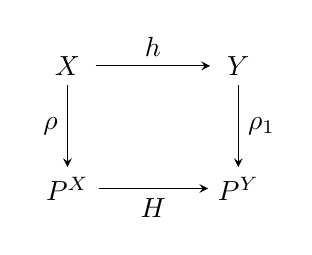
\begin{tikzpicture}
\matrix (m) 
[matrix of math nodes,row sep=3em,column sep=4em,minimum width=2em]
{
X & Y \\
P^X & P^Y \\
};
\path[-stealth]
(m-1-1) edge node [left] {$\rho$} (m-2-1) edge node [above] {$h$} (m-1-2)
(m-2-1) edge node [below] {$H$} (m-2-2)
(m-1-2) edge node [right] {$\rho_1$} (m-2-2);
\end{tikzpicture}
\end{equation*}
Erityisesti $H\vert_{\overline{\rho X}}\colon \overline{\rho X}\rightarrow \overline{\rho_1 Y}$. 
%eli $H\overline{\rho X}\subset \overline{\rho_1 Y}$.
\begin{proof}
Olkoot $X$ ja $Y$ täysin säännöllisiä avaruuksia ja $h\colon X\rightarrow Y$ jatkuva kuvaus. 
%Nyt jokaiselle $g\in I^Y$ löytyy $(g\circ h)\in I^X$, 
Olkoon $g\in I^Y$ kuvaus. Tällöin $(g\circ h)\in I^X$ ja kaavalla 
$h_g\left(\{t_f\}\right)=t_{g\circ h}$ %, $t_f\in I$ 
%$$h_g\left(\prod_{f\in I^X}\{t_f\}\right)=t_{g\circ h}\qquad\text{ kaikilla }t\in I$$ 
voidaan määritellä kuvaus $h_g\colon P^X\rightarrow I_g$. 
Nyt $h_g$ on projektiokuvaus, joka samaistaa yksikkövälit $I_g$ ja $I_{g\circ h}$. 
%Näin ollen tullaan samaistaneeksi yksikkövälit $I_g$ ja $I_{g\circ h}$ projektiokuvauksella $h_g$. 
Kuvaus $h_g$ on jatkuva, joten kaavalla 
$$H\left(\{t_f\}\right)=\{h_g\left(\{t_f\}\right)\},\quad\{t_f\}\in P^X$$ 
voidaan muodostaa jatkuva kuvaus $H\colon P^X\rightarrow P^Y$. 
Nyt kuvauksen $H$ määrittelyn nojalla pätee 
$$(H\circ \rho)(x)=(H ( \rho(x)))=H(\{f(x)\})=\{h_g(\{f(x)\})\}=\{((g\circ h)(x))_g\}$$
ja lauseen \ref{comp_reg_upotus} nojalla
$$(\rho_1\circ h)(x)=\rho_1( h(x))=\{g( h(x))_g\}=\{((g\circ h)(x))_g\}.$$
Näin ollen annettu kaavio kommutoi. 

Kaavion kommutoinnin nojalla $H(\rho X)\subset \rho_1 Y$ 
%Kaavion kommutoinnista seuraa, että $H(\rho (X))\subset \rho_1(Y)$ 
ja näin ollen $\overline{H(\rho X)}\subset \overline{\rho_1 Y}$. 
%ja edelleen $\overline{H(\rho X)}\subset \overline{\rho_1 Y}$. 
Kuvauksen $H$ jatkuvuuden nojalla 
$H(\overline{\rho X})\subset \overline{H(\rho X)}$. 
Nyt $H(\overline{\rho X})\subset\overline{\rho_1 Y}$ 
ja siis $H\vert_{\overline{\rho X}}\colon \overline{\rho X}\rightarrow \overline{\rho_1 Y}$. 
\end{proof}
\end{lause}

\chapter{Kompaktisointi}
Tässä luvussa esitellään topologisen avaruuden kompaktisointi sekä rakennetaan täysin säännöllisen avaruuden Stone-Čech kompaktisointi käyttäen hyväksi edellisen luvun upotusta yksikkövälien tuloon.
Lisätietoja tämän luvun aiheista löytyy kirjasta %Dugundji: Topology 
\cite{Dugu}.

\begin{maar}
Topologisen avaruuden $X$ kompaktisointi on pari $(\hat{X},h)$, 
jossa $\hat{X}$ on kompakti Hausdorff avaruus 
ja $h$ on sellainen homeomorfismi $X\rightarrow h(X)\subset\hat{X}$, 
jolla $h(X)$ on tiheä avaruudessa $\hat{X}$, eli $\overline{ h(X)}=\hat{X}$. 
\end{maar}
\begin{huom}
Usein samastetaan avaruus $X$ ja osajoukko $h(X)\subset\hat{X}$ ja sanotaan, 
että $\hat{X}$ on avaruuden $X$ kompaktisointi. 
\end{huom}

\begin{lem}
Olkoon $X$ täysin säännöllinen avaruus ja $\rho\colon X\rightarrow P^X$ lauseen \ref{comp_reg_upotus} mukainen upotus missä $P^X$ on yksikkövälien tulona kompakti. 
Erityisesti $\overline{\rho X}$ on kompaktin joukon suljettuna osajoukkona kompakti. 
Merkitään $\beta X=\overline{\rho X}$ ja sanotaan, 
että pari $(\beta X,\rho)$ on avaruuden $X$ \emph{Stone-Čech kompaktisointi}.
\end{lem}
\begin{lause}\label{SC-ominaisuus}
Olkoon $X$ täysin säännöllinen avaruus. 
%ja $(\beta X,\rho)$ avaruuden $X$ Stone-Čech kompaktisointi. 
Avaruuden $X$ Stone-Čech kompaktisoinnille $(\beta X,\rho)$ pätee seuraava ominaisuus: 
%Tällöin seuraavat ominaisuudet pätevät:
%1
\begin{itemize}
\item
Jokaiselle kompaktille $Y$ ja jokaiselle jatkuvalle kuvaukselle $f\colon X\rightarrow Y$ on olemassa yksikäsitteinen jatkuva kuvaus $F\colon\beta X\rightarrow Y$ niin, että $f=F\circ \rho$.
\end{itemize}
\begin{proof}
Olkoon $X$ täysin säännöllinen avaruus, $Y$ kompakti avaruus ja 
$f\colon X\rightarrow Y$ jatkuva kuvaus. 
Tällöin lauseen \ref{kommutoiva_kaavio} nojalla on olemassa jatkuva 
kuvaus $\phi\colon \beta X\rightarrow \beta Y$ niin, 
että oheinen kaavio kommutoi.
\begin{equation*}
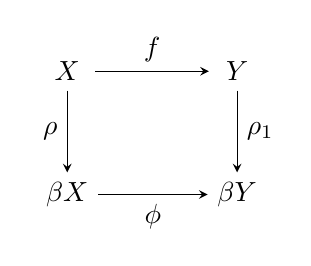
\begin{tikzpicture}
\matrix (m) 
[matrix of math nodes,row sep=3em,column sep=4em,minimum width=2em]
{
X & Y \\
\beta X & \beta Y \\
};
\path[-stealth]
(m-1-1) edge node [left] {$\rho$} (m-2-1) edge node [above] {$f$} (m-1-2)
(m-2-1) edge node [below] {$\phi$} (m-2-2)
(m-1-2) edge node [right] {$\rho_1$} (m-2-2);
\end{tikzpicture}
\end{equation*}
Avaruus $Y$ on kompakti, joten kuvaus $\rho_1\colon Y \rightarrow \beta Y$ on homeomorfismi. 
Näin ollen on olemassa jatkuva käänteiskuvaus $\rho_1^{-1}\colon\beta Y\rightarrow Y$. 
Voidaan nyt valita $F\colon\beta X\rightarrow Y$ asettamalla $F(a)=(\rho_1^{-1}\circ \phi)(a)=\rho_1^{-1}( \phi(a))$ kaikilla $a\in\beta X$.
Nyt $f(x)=(F\circ\rho)(x)$ kaikilla $x\in X$. 
%Lisäksi $\beta X$ on avaruuden $X$ kompaktisointi, joten 
Lisäksi kompaktisoinnin määritelmän nojalla 
$X$ on tiheä joukossa $\beta X$ ja 
näin ollen 
%lemman ??? nojalla 
kuvaus $F$ on yksikäsitteinen. 
\end{proof}
\end{lause}
\begin{lause}
Stone-Čech kompaktisoinnin yksikäsitteisyys. 
Olkoon $X$ täysin säännöllinen avaruus 
%ja $(\beta X,\rho)$ avaruuden $X$ Stone-Čech kompaktisointi. 
%%2 Yksikäsitteisyys. 
%Olkoon
ja $(\hat{X},h)$ sellainen avaruuden $X$ kompaktisointi, 
%Jokainen avaruuden $X$ kompaktisointi $(\hat{X},h)$, 
jolla on lauseen \ref{SC-ominaisuus} kuvaileva ominaisuus. 
Tällöin $\hat{X} $ ja Stone-Čech kompaktisointi $\beta X$ ovat homeomorfisia. 
%Tällöin $\hat{X} $ on homeomorfinen Stone-Čech kompaktisoinnin $\beta X$ kanssa. 
\begin{proof}
Olkoon $X$ täysin säännöllinen avaruus, 
$(\beta X,\rho)$ avaruuden $X$ Stone-Čech kompaktisointi 
ja $(\hat{X},h)$ sellainen avaruuden $X$ kompaktisointi, 
jolla on lauseen \ref{SC-ominaisuus} kuvaileva ominaisuus. 
Samastetaan $X$, $hX$ ja $\rho X$, jolloin voidaan mieltää $X$ joukkojen $\beta X$ ja $\hat{X}$ osajoukoksi. 
Olkoon $i\colon X\rightarrow X$ identtinen kuvaus. 
Nyt lauseen \ref{SC-ominaisuus} ominaisuuden nojalla 
kompaktisoinnille $\beta X$, kompaktille joukolle $\hat{X}$ ja kuvaukselle $i$ 
on olemassa jatkuva kuvaus 
$F\colon\beta X\rightarrow \hat{X}$, 
jolla $F(x)=(F\circ\rho)(x)=i(x)=x$ kaikilla $x\in X$. 
Vastaavasti on olemassa jatkuva kuvaus $G\colon \hat{X}\rightarrow \beta X$,
jolla $G(x)=x$ kaikilla $x\in X$. 
Nyt kuvaukset $(F\circ G)\vert_X$ ja $(G\circ F)\vert_X$ ovat 
identtisiä kuvauksia. 
Lisäksi $X$ on tiheä joukoissa $\beta X$ ja $\hat{X}$, joten 
kuvaukset $F\circ G=1_{\hat{X}}$ ja $G\circ F=1_{\beta X}$ ovat identtisiä kuvauksia. 
Siis kuvaus $F$ on homeomorfismi avaruuksien $\beta X$ ja $\hat{X}$ välille.
\end{proof}
\end{lause}
\begin{lause}
Olkoon $X$ täysin säännöllinen avaruus. 
%ja $(\beta X,\rho)$ avaruuden $X$ Stone-Čech kompaktisointi. 
%3
Stone-Čech kompaktisointi $\beta X$ on laajin 
kompaktisointi avaruudelle $X$: 
%Olkoon $\hat{X}$ avaruuden $X$ kompaktisointi ja 
Jos $\hat{X}$ on avaruuden $X$ kompaktisointi, 
niin $\hat{X}$ on homeomorfinen avaruuden $\beta X$ tekijäavaruuden kanssa. 
%$\sim$ sellainen ekvivalenssirelaatio, jolla $a\sim a'$ jos ja vain jos $F(a)=F(a')$, kun $a,a'\in \beta X$.
%Tällöin kompaktisointi $\hat{X}$ on homeomorfinen tekijäavaruuden 
%$\beta X / \sim$ kanssa. 
%%ekvivalenssirelaatiolla $\sim$, jolla $a\sim a'$ jos ja vain jos $F(a)=F(a')$, $a,a'\in \beta X$.
\begin{proof}
Lauseen \ref{SC-ominaisuus} nojalla on olemassa 
jatkuva kuvaus $F\colon \beta X\rightarrow \hat{X}$, 
jolla $F(x)=x$ kaikilla $x\in X$. 
Avaruus $\beta X$ on kompakti, $\hat{X}$ on Hausdorff ja kuvaus $F$ on jatkuva, joten $F$ on suljettu kuvaus \cite[lause~15.15]{Topo2}.
%Avaruus $\beta X$ on kompakti, joten 
Tällöin kuvajoukko $F(\beta X)\subset\hat{X}$ on suljettu. 
%joka sisältää 
Toisaalta osajoukko $X\subset F(\beta X)$ on tiheä joukossa $\hat{X}$, 
%tiheän osajoukon $X$, 
%Näin ollen 
joten $\overline{X}\subset F(\beta X) = \hat{X}$. 
%ja siten 
Näin ollen kuvaus $F$ on surjektio. 
Kuvaus $F$ on siis suljettu jatkuva surjektio, 
%ja näin ollen 
joten $F$ on samastuskuvaus \cite[lause~8.9]{Topo2}. 

Olkoon $\sim$ sellainen ekvivalenssirelaatio, jolla $a\sim a'$ jos ja vain jos $F(a)=F(a')$, kun $a,a'\in \beta X$. 
Nyt voidaan määritellä kuvaus 
$F_{\sim}\colon \beta X /\sim\,\rightarrow \hat{X}$, jolla $F_{\sim}([a])=F(a)$. 
%Kuvaus $F_{\sim}$ on injektio, sillä jos $x,y\in \beta X$ ja $[x]\neq [y]$ niin $F_{\sim}([x])=F(x)\neq F(y)=F_{\sim}([y])$. 
%TODO tästä eteenpäin topo2:sta samastuskuvaus määritelmineen ja tekijätopologian tuloksien avulla todistuksen loppuosa
%Olkoon $\rho\colon \beta X\rightarrow \beta X/\sim$ projektiokuvaus, 
%jolla $\rho(a)=[a]$ kaikilla $a\in\beta X$. Kuvaus $F$ on jatkuva, 
%$\rho$ on projektiokuvauksena jatkuva ja $F=F_{\sim}\circ \rho$, 
%joten $F_{\sim}$ on jatkuva. 
%
%(Puuttuu perustelu miksi $F_{\sim}$ on avoin kuvaus.)
%
Kuvaus $F$ on samastuskuvaus, joten kuvaus $F_{\sim}$ %\colon \beta X /\sim\,\rightarrow \hat{X}$ 
on homeomorfismi \cite[lause~9.10]{Topo2}.
Siis kompaktisointi $\hat{X}$ on homeomorfinen tekijäavaruuden 
$\beta X / \sim$ kanssa. 
\end{proof}
\end{lause}


%
%\newpage
%\begin{huom}
%\end{huom}
%\begin{lause}
%\end{lause}
%\begin{maar}
%\end{maar}
%\begin{kor}
%\end{kor}
%\begin{esim}
%\end{esim}
%\begin{lem}
%\end{lem}
%
%\chapter{Universaali uniforminen rakenne}
%\begin{maar}
%\emph{Universaali uniformiteetti.} 
%Olkoon $(X,\T)$ uniformisoituva topologinen avaruus ja 
%$(f_i)_{i\in I}$ kaikkien jatkuvien pseudometriikkojen perhe, 
%jossa $f_i\colon X\times X\rightarrow [0,\infty]$ 
%kaikilla $i\in I$. 
%Perheen $(f_i)_{i\in I}$ määrittelemä uniformiteetti on 
%avaruuden $(X,\T)$ \emph{universaali uniformiteetti} (universal uniformity), 
%jota merkitsemme symbolilla $\U_0$. 
%\end{maar}
%\begin{lause}
%Uniformisoituvan topologisen avaruuden $(X,\T)$ universaali uniformiteetti $\U_0$ on hienoin niistä uniformiteeteista, jotka ovat yhteensopivia topologian $\T$ kanssa. 
%\begin{proof}
%Olkoon $(X,\T)$ uniformisoituva topologinen avaruus ja 
%$\U_0$ avaruuden $(X,\T)$ universaali uniformiteetti. 
%Olkoon lisäksi $\U$ joukon $X$ uniformiteetti, 
%joka on yhteensopiva topologian $\T$ kanssa. 
%
%
%
%
%%TODO
%Kesken.
%\end{proof}
%\end{lause}
%\begin{lause}
%Olkoon $(X,\T)$ uniformisoituva topologinen avaruus, 
%$\U_0$ avaruuden $(X,\T)$ universaali uniformiteetti, 
%%$\U$ joukon $X$ uniformiteetti, joka on yhteensopiva topologian $\T$ kanssa. 
%%Jos $Y$ on uniforminen avaruus ja $f\colon X\rightarrow Y$ 
%%Olkoon 
%$(Y,\U)$ uniforminen avaruus ja $f\colon X\rightarrow Y$ 
%%jatkuva kuvaus (topologian $\T$ suhteen). 
%kuvaus. 
%Jos kuvaus $f$ on jatkuva uniformiteetin $\U$ määräämän topologian suhteen, %(topologian $\T$ suhteen), 
%niin $f$ on myös tasaisesti jatkuva. %(uniformiteetin $\U_0$ suhteen). 
%%Kuvaus $f$ on tasaisesti jatkuva (uniformiteetin $\U$ suhteen), 
%%jos ja vain jos uniformiteetti $\U$ on 
%%avaruuden $(X,\T)$ universaali uniformiteetti. 
%\begin{proof}
%%%Osoitetaan väitteen implikaatio molempiin suuntiin.
%%%\begin{enumerate}
%%%\item[$\Rightarrow$]
%%%Olkoon kuvaus $f$ tasaisesti jatkuva. 
%%%\item[$\Leftarrow$]
%%Olkoon uniformiteetti $\U$ on 
%%avaruuden $(X,\T)$ universaali uniformiteetti. 
%%Tällöin uniformiteetin $\U$ indusoiman topologian $\T$ ympäristöt ovat muotoa $ V(x)$, jossa $V\in\T$ ja $x\in X$
%%%\end{enumerate}
%%TODO
%Olkoon $(X,\T)$ uniformisoituva topologinen avaruus ja 
%$\U_0$ avaruuden $(X,\T)$ universaali uniformiteetti. 
%Olkoon lisäksi $(Y,\U)$ uniforminen avaruus, $\T_{\U}$ uniformiteetin $\U$ määräämä topologia avaruudelle $Y$ ja $f\colon X\rightarrow Y$ 
%jatkuva kuvaus (topologian $\T_{\U}$ suhteen). 
%
%Olkoon $V\in \U$ lähistö ja $y\in Y$ alkio. 
%Tällöin $V(y)$ on alkion $y$ ympäristö topologiassa $\T_{\U}$. 
%Kuvaus $f$ on jatkuva, 
%joten alkukuva $f^\leftarrow V(y)\subset X$ on topologian $\T$ ympäristö. 
%Olkoon $x\in f^\leftarrow V(y)$, eli $f(x)\in V(y)$. 
%Oletetaan, että $x'\in X$ on sellainen alkio, jolla $f(x')= y$.
%Tällöin $(x,x')\in f^\leftarrow V$ 
%ja $(f(x),y)\in V$. 
%
%
%Kesken. Puuttuu osoitus, että on olemassa lähistö $W\in\U_0$ niin, että $(x,x')\in W$ ja $W\subset f^\leftarrow V$.
%
%
%%niin $f$ on myös tasaisesti jatkuva. 
%%Kesken.
%\end{proof}
%\end{lause}
%\begin{lause}
%Olkoon $(X,\T)$ uniformisoituva topologinen avaruus ja 
%$\U_0$ avaruuden $(X,\T)$ universaali uniformiteetti. 
%Olkoon tällöin  
%$\U$ sellainen joukon $X$ uniformiteetti, 
%joka on yhteensopiva topologian $\T$ kanssa ja 
%jolla avaruus $(X,\U)$ on täydellinen. 
%Tällöin myös $(X,\U')$ on täydellinen jokaisella 
%uniformiteetilla $\U'$, jolla 
%$\U\subset\U'\subset\U_0$.
%\begin{proof}
%%Cauchy-filtterit ovat samoja.
%%TODO
%Puuttuu.
%\end{proof}
%\end{lause}
%%
%%
%\chapter{Hausdorff uniforminen avaruus}
%Tässä luvussa määritellään Hausdorff uniformiset avaruudet ja 
%esitetään niiden ominaisuuksia, 
%oleellisimpana täydelliseen Hausdorff uniformiseen avaruuteen laajentaminen.
%\begin{maar}
%%Olkoon $X$ joukko ja $\U$ uniformiteetti joukolle $X$. 
%%Olkoon lisäksi $(f_i)_{i\in I}$ sellainen pseudometriikkaperhe, joka määrittelee uniformiteetin $\U$. 
%%Uniformiteetti $\U$ on \emph{Hausdorff}, jos kaikille alkioille $x,y\in X$ on 
%%olemassa pseudometriikka $f_i\in(f_i)_{i\in I}$, 
%%jolla ehdosta $x\neq y$ seuraa $f_i(x,y)\neq 0$. 
%Olkoon $(X,\U)$ uniforminen avaruus ja $(f_i)_{i\in I}$ sellainen 
%pseudometriikkaperhe, joka määrittelee uniformiteetin $\U$. 
%Uniformiteetti $\U$ on \emph{Hausdorff}, jos jokaisilla alkioilla 
%$x,y\in X$ ehdosta $x\neq y$ seuraa $f_k(x,y)\neq 0$ 
%jollain pseudometriikalla $f_k\in(f_i)_{i\in I}$. 
%Erityisesti, jos uniformiteetti $\U$ on Hausdorff 
%ja yhden pseudometriikan $f$ määrittelemä, 
%niin $f(x,y)\neq 0$ kaikilla $x,y\in X$, $x\neq y$.
%\end{maar}
%\begin{huom}
%%Olkoon $X$ joukko ja $\U$ pseudometriikkaperheen $(f_i)_{i\in I}$ 
%%määrittelemä uniformiteetti. 
%%Uniformiteetti $\U$ ei ole Hausdorff, jos on olemassa sellaiset alkiot $x,y\in X$, joilla $x\neq y$ ja $f_k(x,y)=0$ kaikilla $f_k\in (f_i)_{i\in I}$.
%Olkoon $X$ joukko ja $(f_i)_{i\in I}$ pseudometriikkaperhe joukolle $X$. 
%Pseudometriikkaperheen $(f_i)_{i\in I}$ määrittelemä uniformiteetti ei ole 
%Hausdorff, jos on olemassa sellaiset alkiot $x,y\in X$, 
%joilla $x\neq y$ ja $f_k(x,y)=0$ kaikilla $f_k\in (f_i)_{i\in I}$.
%\end{huom}
%%\begin{lem}
%%Olkoon $X$ uniforminen avaruus, $A\subset X$ epätyhjä osajoukko 
%%ja $f$ pseudometriikka joukolle $X$. 
%%Tällöin pseudometriikan rajoittuma 
%%$f|_A\colon A\times A\rightarrow [0,\infty]$ kaavalla $ f|_A(x)=f(x)$ 
%%kaikilla $x\in A\times A$ 
%%on pseudometriikka joukolle $A$. \qed
%%\end{lem}
%%\begin{lem}
%%Olkoon $X$ uniforminen avaruus, $A\subset X$ epätyhjä osajoukko 
%%ja $(f_i)_{i\in I}$ pseudometriikkaperhe, 
%%joka määrää joukon $X$ uniformiteetin. 
%%Tällöin joukon $X$ uniformiteetti määrää joukolle $A$ saman uniformiteetin 
%%kuin pseudometriikkaperhe $(f_i|_A)_{i\in I}$.
%%\end{lem}
%\begin{lause}\label{complete}
%Olkoon $X$ uniforminen avaruus. 
%Tällöin on olemassa täydellinen (com\-plete) Hausdorff 
%uniforminen avaruus $\hat X$ ja tasaisesti jatkuva 
%kuvaus $i\colon X\rightarrow\hat X$, jolle pätee seuraava ominaisuus:
%\begin{enumerate} [label=(P),ref=(P)]
%%\begin{enumerate}
%\item %[(P)] 
%\label{ominaisuusP}
%Olkoon $Y$ täydellinen Hausdorff uniforminen avaruus 
%ja $f\colon X\rightarrow Y$ tasaisesti jatkuva kuvaus. 
%Tällöin on olemassa yksikäsitteinen tasaisesti 
%jatkuva $g\colon \hat X\rightarrow Y$, 
%jolla pätee $f=g\circ i$.
%\end{enumerate}
%Tällöin sanotaan, että avaruus $\hat X$ on avaruuden $X$ \emph{Hausdorff täydennys}.
%\begin{proof}
%%TODO
%Puuttuu.
%\end{proof}
%\end{lause}
%\begin{lause}
%Olkoon $X$ uniforminen avaruus ja $\hat X$ Hausdorff täydennys avaruudelle $X$. 
%Olkoon lisäksi $X_1$ täydellinen Hausdorff 
%uniforminen avaruus ja $i_1\colon X\rightarrow X_1$
%tasaisesti jatkuva kuvaus, jolla on ominaisuus \ref{ominaisuusP}. 
%Tällöin on olemassa yksikäsitteinen isomorfismi $\varphi\colon\hat X\rightarrow X_1$, jolla pätee $i_1=\varphi\circ i$.
%\begin{proof}
%%TODO
%Puuttuu.
%\end{proof}
%\end{lause}
%\begin{kor}
%Olkoon $X$ on Hausdorff uniforminen avaruus ja $\hat X$ määritelmän \ref{complete} mukainen täydellinen Hausdorff uniforminen avaruus. 
%Niin sanottu kanoninen kuvaus $i\colon X\rightarrow\hat X$ määrää 
%isomorfismin $X\rightarrow X'$, jossa $X'\subset \hat X$ on tiheä joukossa $\hat X$.
%\begin{proof}
%%TODO
%Puuttuu.
%\end{proof}
%\end{kor}
%\begin{lause}
%Olkoon $X$ ja $Y$ uniformeja avaruuksia ja $i_X\colon X\rightarrow\hat{X}$ ja $i_Y\colon Y\rightarrow\hat{Y}$ kanonisia kuvauksia. 
%Jokaiselle tasaisesti jatkuvalle kuvaukselle $f\colon X\rightarrow Y$ 
%löytyy yksikäsitteinen tasaisesti jatkuva kuvaus $\hat{f}\colon \hat{X}\rightarrow \hat{Y}$, jolla oheinen diagrammi kommutoi. 
%%X--->Y
%%|    |
%%v    v
%%^X->^Y
%\begin{equation*}
%\begin{tikzpicture}
%\matrix (m) 
%[matrix of math nodes,row sep=3em,column sep=4em,minimum width=2em]
%{
%X & Y \\
%\hat{X} & \hat{Y} \\
%};
%\path[-stealth]
%(m-1-1) edge node [left] {$i_X$} (m-2-1) edge node [above] {$f$} (m-1-2)
%(m-2-1) edge node [below] {$\hat{f}$} (m-2-2)
%(m-1-2) edge node [right] {$i_Y$} (m-2-2);
%\end{tikzpicture}
%\end{equation*}
%\begin{proof}
%%TODO
%Puuttuu.
%\end{proof}
%\end{lause}
%\chapter{Kompakti uniforminen avaruus}
%
%\begin{maar}
%Olkoon $(X,\T)$ täysin säännöllinen topologinen avaruus 
%ja $\U$ topologian $\T$ kanssa yhteensopiva uniformiteetti. 
%Olkoon $(f_i)_{i\in I}$ kaikkien uniformiteetin $\U$ suhteen tasaisesti jatkuvien kuvausten $f_i\colon X\rightarrow [0,1]$ perhe. 
%Tällöin merkitään symbolilla $\U^*$ sitä uniformiteettia, 
%joka on karkein niistä uniformiteeteista, 
%joilla kaikki kuvausperheen $(f_i)_{i\in I}$ 
%kuvaukset %$f\colon X\rightarrow [0,1]$ 
%ovat tasaisesti jatkuvia. 
%%joilla kaikki uniformiteetin $\U$ suhteen tasaisesti jatkuvat 
%%kuvaukset $f\colon X\rightarrow [0,1]$ ovat tasaisesti jatkuvia. 
%%uniformiteetin $\U^*$ suhteen. 
%\end{maar}
%
%\begin{lause}
%Olkoon $(X,\T)$ täysin säännöllinen topologinen avaruus. 
%%ja $\U$ topologian $\T$ kanssa yhteensopiva uniformiteetti. 
%Tällöin uniformiteetti $\U^*$ on Hausdorff ja yhteensopiva topologian $\T$ kanssa. 
%\begin{proof}
%%TODO
%Puuttuu.
%\end{proof}
%\end{lause}
%
%\begin{maar}
%%\emph{Esikompakti avaruus. Uniformisen avaruuden kompaktius.} 
%Uniforminen avaruus $X,\U$ on \emph{esikompakti}, 
%jos sen Hausdorff täydennys %(completion) 
%$\hat{X}$ on kompakti. 
%Epätyhjä osajoukko $A\subset X$ on esikompakti, jos $(A,\U\vert _A)$ on esikompakti. 
%(Rajoitettu uniformiteetti $\U\vert _A=\{U\cap (A\times A)\mid U\in\U\}$.)
%\end{maar}
%
%\begin{lause}
%Olkoon $(X,\T)$ täysin säännöllinen topologinen avaruus. 
%%ja $\U$ topologian $\T$ kanssa yhteensopiva uniformiteetti. 
%Tällöin avaruus $(X,\U^*)$ on esikompakti.
%\begin{proof}
%%TODO
%Puuttuu.
%\end{proof}
%\end{lause}
%
%\begin{lause}
%Olkoon $(X,\T)$ täysin säännöllinen topologinen avaruus 
%ja $\U$ topologian $\T$ kanssa yhteensopiva uniformiteetti. 
%Olkoon $(K,\T')$ kompakti (topologinen) avaruus ja 
%$\U_{\T'}$ topologian $\T'$ kanssa yhteensopiva uniformiteetti. 
%Olkoon $f\colon X\rightarrow K$ kuvaus, joka on tasaisesti jatkuva uniformiteetin $\U$ suhteen. 
%%$f\colon (X,\U)\rightarrow (K,\U_{\T'})$ tasaisesti jatkuva kuvaus. 
%%Tällöin myös $f\colon (X,\U^*)\rightarrow (K,\U_{\T'})$ on 
%%tasaisesti jatkuva. 
%Tällöin kuvaus $f$ on tasaisesti jatkuva myös uniformiteetin $\U^*$ suhteen. 
%\begin{proof}
%%TODO
%Puuttuu.
%\end{proof}
%\end{lause}
%
%\begin{kor}
%Uniformiteetti $\U^*$ on hienoin niistä topologian $\T$ 
%kanssa yhteensopivista uniformiteeteista $\U$, 
%joilla $(X,\U)$ on esikompakti. 
%\begin{proof}
%%TODO
%Puuttuu.
%\end{proof}
%\end{kor}
%
%\begin{maar}
%\emph{Stone–Čech kompaktisointi.}
%Olkoon $(X,\T)$ täysin säännöllinen topologinen avaruus ja 
%$\U_0$ avaruuden $(X,\T)$ universaali uniformiteetti. 
%Olkoon $\U^{*}_{0}$ karkein uniformiteetti, 
%jolla kaikki jatkuvat kuvaukset $f_i\colon X\rightarrow [0,1]$ 
%ovat tasaisesti jatkuvia. 
%Olkoon $\beta X$ avaruuden $(X,\U^{*}_{0})$ Hausdorff täydennys.
%%kompakti (topologinen) avaruus, 
%%joka saadaan täydentämällä avaruus $(X,\U^{*}_{0})$.
%Avaruutta $\beta X$ sanotaan avaruuden $(X,\T)$ 
%Stone–Čech kompaktisoinniksi.
%\end{maar}
%
%%\begin{lause}
%%Olkoon $(X,\T)$ täysin säännöllinen topologinen avaruus ja 
%%$(K,\T')$ kompakti topologinen avaruus. 
%%Tällöin jokainen jatkuva kuvaus $f\colon X\rightarrow K$, voidaan laajentaa kuvaukseksi $f'\colon \beta X\rightarrow K$.
%%\begin{proof}
%%%TODO
%%Puuttuu.
%%\end{proof}
%%\end{lause}
%
%


%\begin{huom}
%\end{huom}
%\begin{lause}
%\end{lause}
%\begin{maar}
%\end{maar}
%\begin{kor}
%\end{kor}
%\begin{esim}
%\end{esim}
%\begin{lem}
%\end{lem}
\begin{thebibliography}{9}

\bibitem{Eom1}
Nicolas Bourbaki: General Topology Part 1, 1.\ painos, Hermann, 1966.

\bibitem{Eom2}
Nicolas Bourbaki: General Topology Part 2, 1.\ painos, Hermann, 1966.

%\bibitem{Bor}
%Karol Borsuk: Theory of retracts, %n.\ painos, 
%Państwowe Wydawn. Naukowe, 1967.
%
%\bibitem{Topo1}
%Jussi Väisälä: Topologia I, 4.\ korjattu painos, Limes ry, 2007.
%
\bibitem{Topo2}
Jussi Väisälä: Topologia II, 2.\ korjattu painos, Limes ry, 2005.

\bibitem{Dugu}
James Dugundji: Topology, 11.\ korjattu painos, Allyn and Bacon, 1976.

%\bibitem{Hei}
%Juha Heinonen: Geometric embeddings of metric spaces, luentomoniste, Jyväskylän yliopisto, 2003
%Sheldon (not really) Ross: A First Course in Probability, 5th edition, Prentice-Hall, 1998.

%\bibitem{Tuo}
%Pekka (not really) Tuominen: Todennäköisyyslaskenta I, 5.\ painos, Limes ry, 2000.

\end{thebibliography}

\end{document}
